% !TEX encoding = UTF-8 Unicode
\documentclass[a4paper, 12pt]{report}

\usepackage[utf8]{inputenc} % keyboard input encoding
\usepackage[T1]{fontenc} %font encoding (accents)
\usepackage[english]{babel} %language
\usepackage{lmodern, textcomp} %fonts
\usepackage[left=1.5cm, right=1.5cm, top=2cm, bottom=2cm, headheight = 15pt]{geometry} %mise en page, margin
\usepackage{fancyhdr} %headings
\pagestyle{fancy}
\fancyhead[L]{\footnotesize Loïc Dubois}
\fancyhead[C]{\footnotesize Formation Control of Multiple Small Quadrotors by Using MPC}
\fancyhead[R]{\footnotesize Shinshu University}
\usepackage{amsmath, amssymb} %math
\usepackage{mathtools} %Fixes/improves amsmath
\usepackage{gensymb} %generic symbols
\usepackage[super]{nth} % 1st, 2nd, ...
\usepackage{graphicx, subfig} %sub-figures
\usepackage{array} %tables
\usepackage{hhline} %double horizontal line
\usepackage{caption} %caption figures and tables
\captionsetup[table]{skip=6pt} %caption format for table
\usepackage{listings} %include code
\usepackage{color} %add colors
\definecolor{mygreen}{rgb}{0,0.6,0}
\definecolor{mygray}{rgb}{0.5,0.5,0.5}
\definecolor{mymauve}{rgb}{0.58,0,0.82}
\usepackage[toc,page]{appendix} %appendices
\usepackage{pdfpages} %include pdf

% arabic sections for appendices
\renewcommand{\thesection}{\arabic{section}}

% norm of a vector
\newcommand\norm[1]{\left\lVert#1\right\rVert}

\makeatletter
\renewcommand*\env@matrix[1][*\c@MaxMatrixCols c]{%
  \hskip -\arraycolsep
  \let\@ifnextchar\new@ifnextchar
  \array{#1}}
\makeatother
\begin{document}
%---------------------------------------------------------------------------------------
%	TITLE
%----------------------------------------------------------------------------------------
\begin{titlepage}
\newcommand{\HRule}{\rule{\linewidth}{0.5mm}} % Defines a new command for the horizontal lines, change thickness here
\center
 
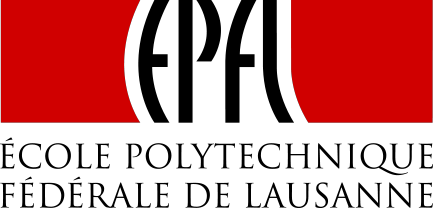
\includegraphics[width=5cm,height=2.4cm]{logo/EPFL.png}
\hspace{7cm}

\includegraphics[width=5cm,height=2.4cm]{logo/Shinshu.png}\\
\vspace{1cm}
\textsc{\large Laboratoire de Systèmes Robotiques, EPFL}\\[0.3cm] 
\textsc{\Large And}\\[0.3cm] 
\textsc{\large Faculty of Textile Science and Technology, Shinshu University}\\[0.5cm] % Major heading such as course name
\vspace{3cm}

{ \huge \bfseries Projet de Master 2017\\
\large Section de Microtechnique\\[1.5cm]
\HRule \\[0.4cm]
\LARGE Formation Control of Multiple Small Quadrotors by Using Model Predictive Control} % Title of your document
\HRule \\[1.5cm]
 
\Large Loïc \textsc{Dubois}\\ % Your name
\vspace{2.5cm}

\begin{minipage}[t]{0.4\textwidth}
\begin{flushleft} \large
\emph{Professors:} \\
Hannes \textsc{Bleuler}\\ % Supervisor's Name
Satoshi \textsc{Suzuki}\\ % Supervisor's Name
\end{flushleft}
\end{minipage}
~
\begin{minipage}[t]{0.4\textwidth}
\begin{flushright} \large
\emph{Assistant:} \\
Romain \textsc{Baud}\\ % Assistant's Name
\end{flushright} 
\end{minipage}\\[3cm]

{\large \today}\\ % Date, change the \today to a set date if you want to be precise


\vfill % Fill the rest of the page with whitespace

\end{titlepage}

\newpage
$\ $
\thispagestyle{empty}
%---------------------------------------------------------------------------------------
%	PRESENTATION SHEET
%----------------------------------------------------------------------------------------
\newpage
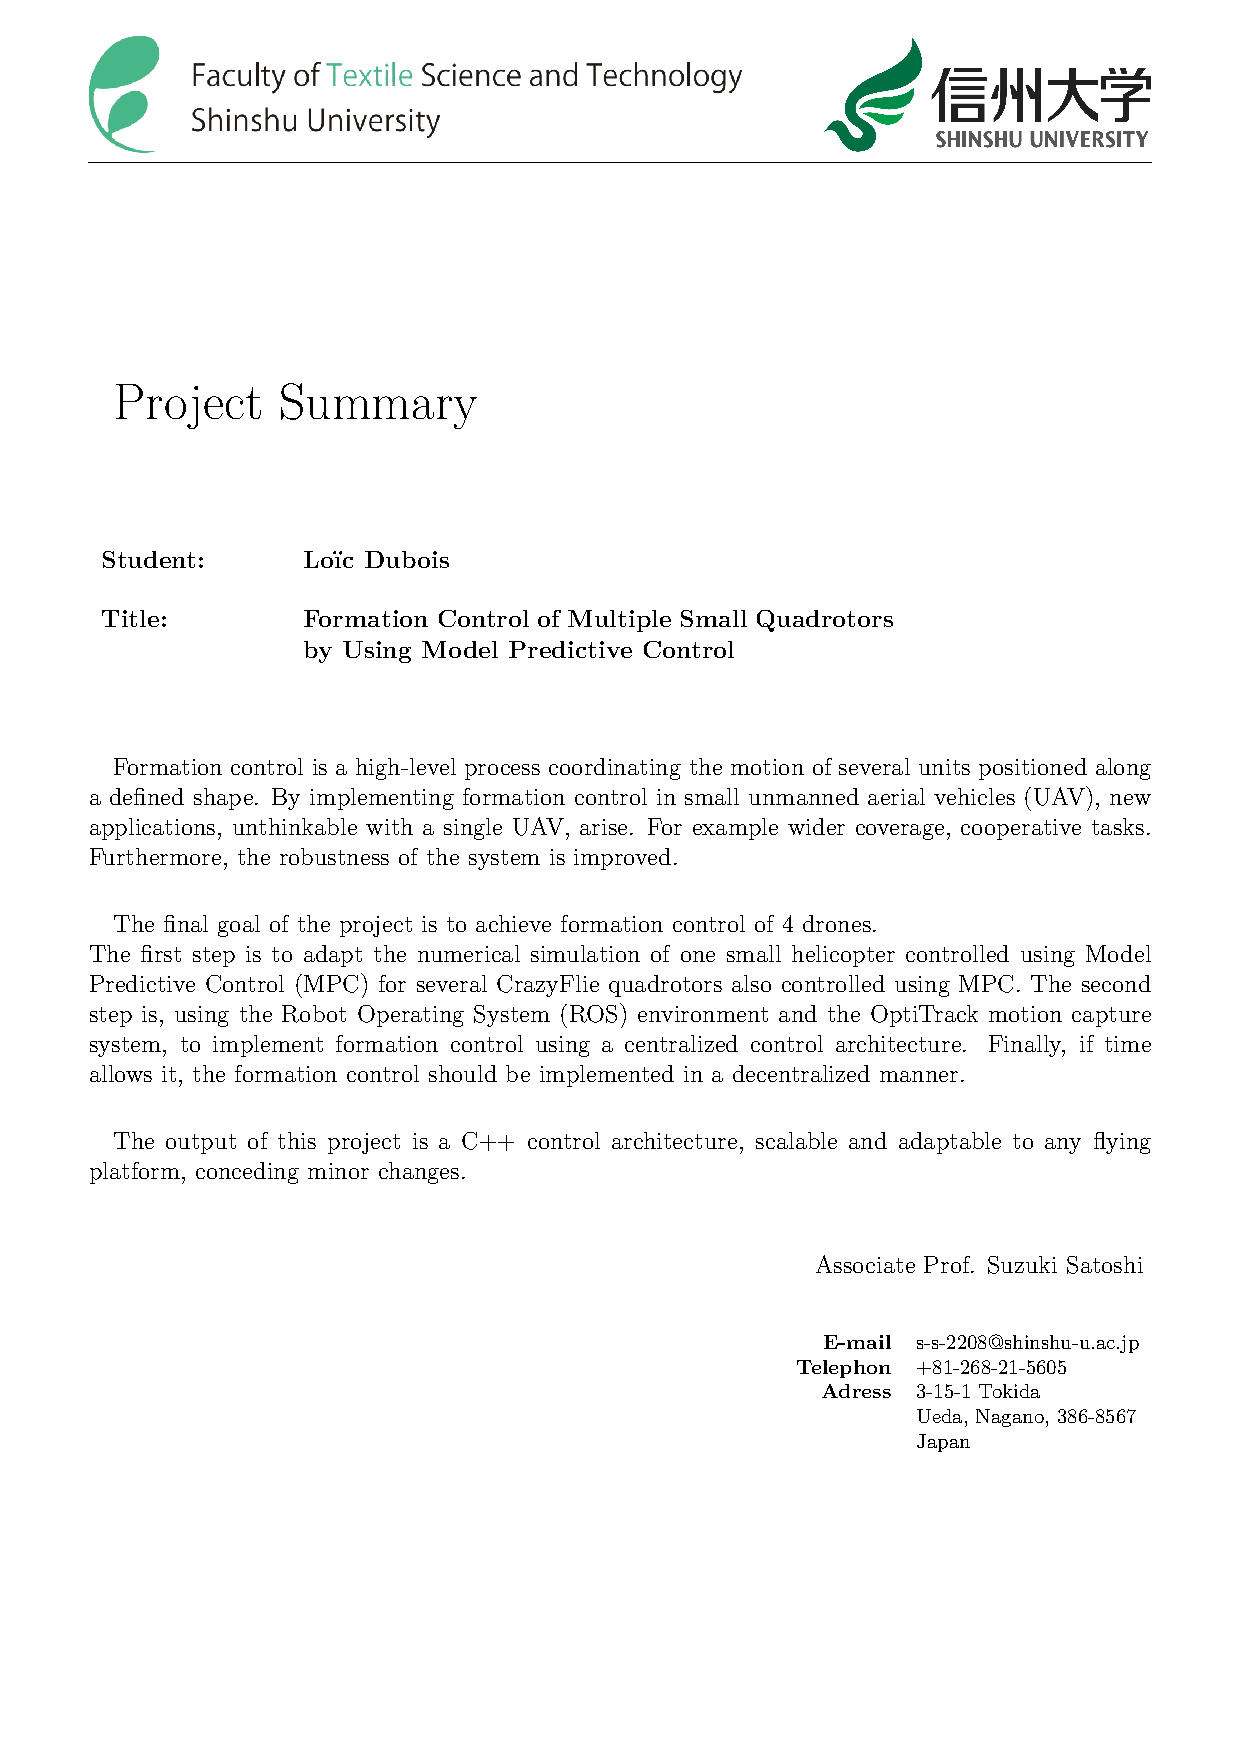
\includepdf{Presentation_sheet/Presentation_sheet.pdf}
\thispagestyle{empty}
\newpage
$\ $
\thispagestyle{empty}
%---------------------------------------------------------------------------------------
%	SUMMARY
%----------------------------------------------------------------------------------------
\newpage
%\includepdf{Presentation_project.pdf}
\textcolor{red}{SUMMARY - To be included - Template: c.f.: Project instructions, STI-MT website}
\thispagestyle{empty}
\newpage
$\ $
\thispagestyle{empty}
%---------------------------------------------------------------------------------------
%	TOC
%----------------------------------------------------------------------------------------
\newpage
\tableofcontents
\thispagestyle{empty}

%---------------------------------------------------------------------------------------
%	REPORT
%----------------------------------------------------------------------------------------
\newpage
% Numbering style
\pagenumbering{roman} 

\section*{Symbols and Abbreviations}
\addcontentsline{toc}{section}{Symbols and Abbreviations}
\subsection*{Symbols}
\begin{table}[h]
\centering
\begin{tabular}{p{8cm} p{8cm}}
$v$ \dotfill & A scalar \\
$\dot v$ \dotfill & First-order time derivative of scalar $v$ \\
$ \ddot v$ \dotfill & Second-order time derivative scalar $v$\\
$c_{\alpha}$ \dotfill & Cosinus of angle $\alpha$ \\
$s_{\alpha}$ \dotfill & Sinus of angle $\alpha$ \\
$\boldsymbol{v}$ \dotfill & A vector in world frame \\
$\boldsymbol{v}_B$ \dotfill & A vector in body frame \\
$\norm{\boldsymbol{v}}$ \dotfill & $L^2$ norm of vector $\boldsymbol{v}$ \\
$\boldsymbol{v}_{i:j}$ \dotfill & Sub vector from composant \emph{i} to \emph{j} of vector $\boldsymbol{v}$\\
$V$ \dotfill & A matrix \\
$V^T,\boldsymbol{v}^T$ \dotfill & Transpose of a matrix $V$ or a vector $\boldsymbol{v}$ \\
$\phi$ \dotfill & Roll angle \\
$\theta$ \dotfill & Pitch angle \\
$\psi$ \dotfill & Yaw angle \\
$\boldsymbol{x}$ \dotfill & State vector \\
$\boldsymbol{u}$ \dotfill & Input vector \\
$\boldsymbol{x}_s$, $\boldsymbol{u}_s$ \dotfill & Working point subscript \\
$\boldsymbol{x}_r$, $\boldsymbol{u}_r$ \dotfill & Reference subscript \\
$A$ \dotfill & A matrix \\
$B$ \dotfill & B matrix \\
$C$ \dotfill & C matrix \\
$D$ \dotfill & D matrix \\
\end{tabular}
\end{table}

\subsection*{Abbreviations}
\begin{table}[h]
\centering
\begin{tabular}{p{8cm} p{8cm}}
MPC \dotfill & Model Predictive Control \\
ROS \dotfill & Robot Operating System \\
GMRES \dotfill & Generalized Minimum Residual method \\
C/GMRES \dotfill & Continuation-GMRES method \\
FPS \dotfill	 & Frame Per Second \\
PWM \dotfill	 & Pulse Width Modulation \\
\end{tabular} 
\end{table}

\newpage
\addcontentsline{toc}{section}{\listtablename}
\listoftables

\newpage
\addcontentsline{toc}{section}{\listfigurename}
\listoffigures

\newpage
% paragraph indentation and spacing
\setlength{\parskip}{1.5em}
\setlength{\parindent}{1em}
% Numbering style
\pagenumbering{arabic} 
\setcounter{page}{1}

\section{Introduction}
Build on \cite{Suzuki2014}

\newpage
\section{Setup}
\textcolor{red}{WHOLE SETUP PRESENTATION}
\begin{figure}[htbp]
\centering
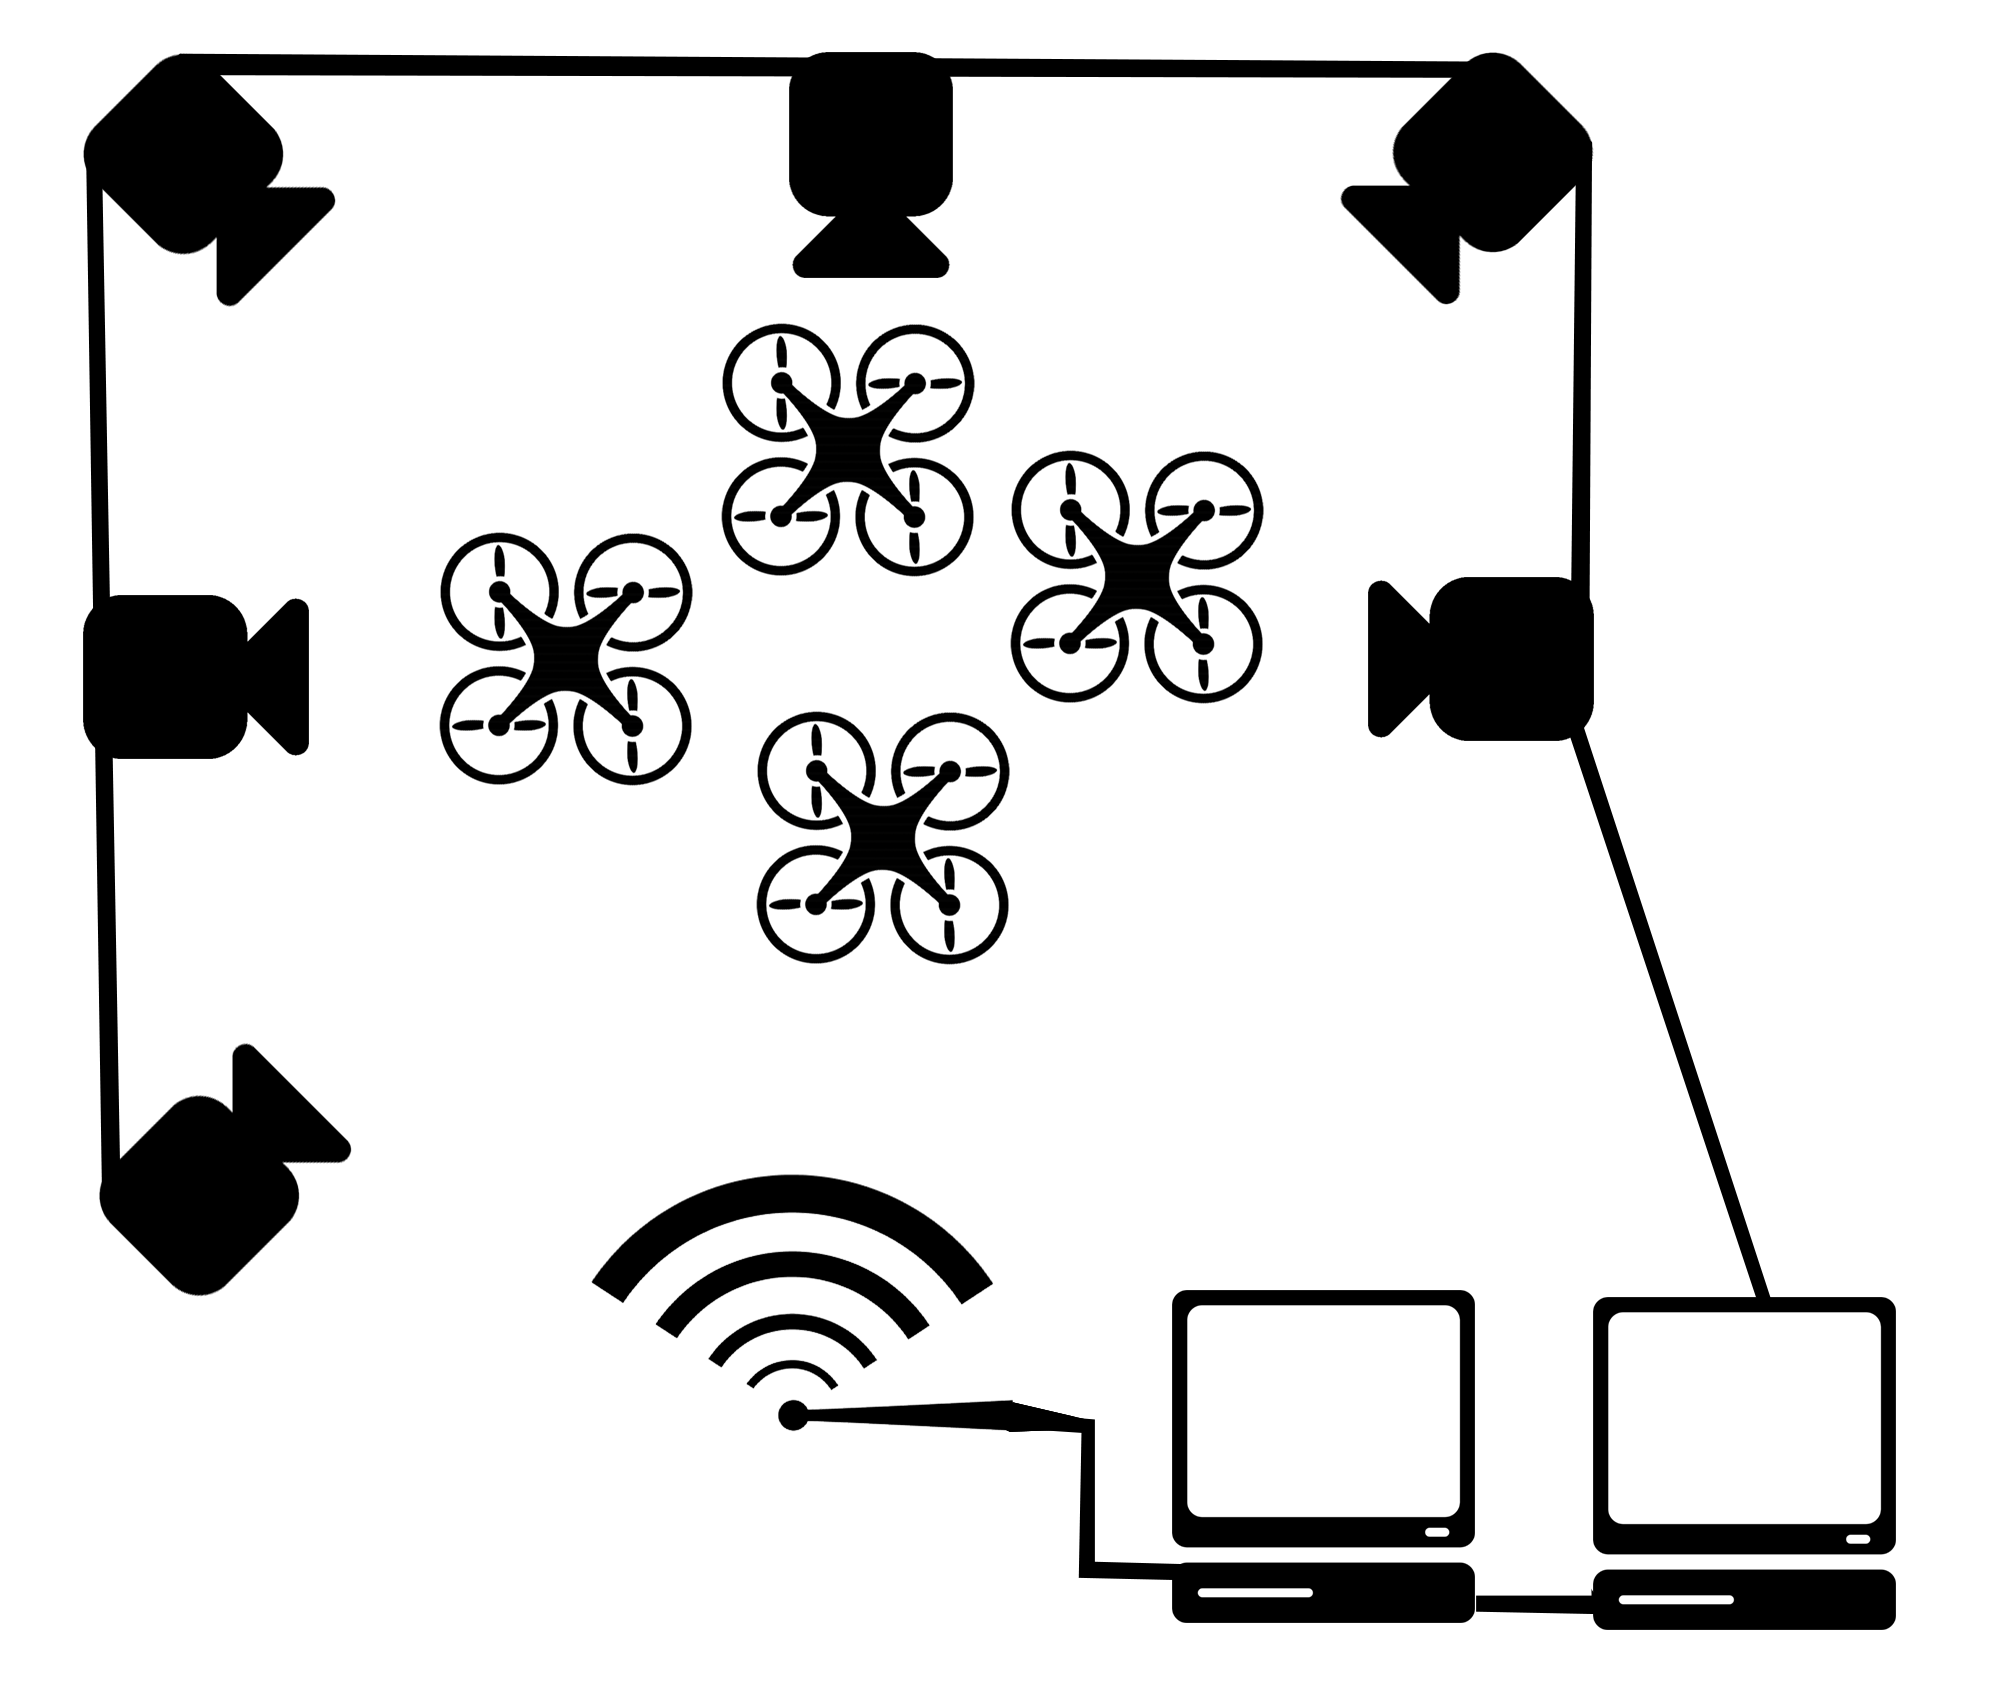
\includegraphics[width=.7\textwidth]{Images/setup}
\caption{Overview of the complete setup}
\label{fig:setup}
\end{figure}
The setup for this project is the same as the one used in \cite{Suzuki2014}. 

\subsection{Crazyflie 2.0 Quadrotor}
The Crazyflie 2.0 (or, from now on, simply CrazyFly) is the second model of small quadrotors (or quadcopter or, simply, quad) developed by Swedish company, BitCraze \cite{bitcraze}. Its length of 92 millimeters from rotor to rotor and its weight of 27 grams make it a safe indoor flying machine. Its on-board battery allows flights up to 7 minutes. Flights that can be controlled thanks to an on-board long-range radio receiver and the appropriate emitter, the CrazyRadio PA or thanks to a Bluetooth LE (low-energy) connexion and a smartphone with the dedicated application. The quadrotor is also equipped with different sensors, including a IMU with a 3-axis high-performance MEMs gyros and accelerometers as well as a 3-axis magnetometer and a barometer.

The Crazyflie 2.0 runs on an open source firmware, available on BitCraze website\cite{bitcraze}, which makes an ideal tool for experimentation on control, estimation, navigation or algorithm validation. The code can be adapted, modified or improved without restrictions. Moreover we can log firmware variables up to 100 Hz and export them to a CSV file, which can be decrypted by Matlab.

\begin{figure}[htbp]
\centering
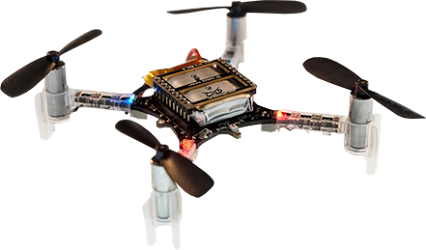
\includegraphics[width=.4\textwidth]{Images/crazyflie}
\captionsetup[subfloat]{labelformat=empty}
\subfloat[Picture from \cite{bitcraze}]{\hspace{\linewidth}}
\caption{The CrazyFlie quadrotor from BitCraze}
\label{fig:cf}
\end{figure}

\subsubsection{Firmware}
A description of the core control C modules is given in section~\ref{sec:innerControl}. Note that the current firmware allows to log state and/or sensor data at a maximal rate of 100 Hz.

\subsection{Robot Operating System}
\textcolor{red}{A ECRIRE}
\subsection{OptiTrack Motion Capture System}
The motion capture system consists, on one side, of eight Prime 13 cameras from OptiTrack and, on the other side, Motive:Tracker, a motion analysis software also from OptiTrack, capable of performing all steps from calibration to the motion capture itself.
This system allow a frame rate of 240 FPS and capture the drone position and attitude, or orientation. \textcolor{red}{Specs Camera: buffer size and length}.

\newpage

\section{Quadrotor dynamics}
A quadrotor can fly in two different configurations, they are commonly called $+$ (plus) and $\times$ (cross). In a $+$ configuration. The X- and the Y-axes are aligned with two perpendicular arms, the control is easier because only two propellers require to have their speed changed to move along a principal axis. On the other side, a $\times$ configuration require all the propellers to change their speed. However the variation of speed per motor is important. In the following section, all dynamics equations are derived for a $+$ configuration. To fly in $\times$, minor changes have to be performed.

\subsection{State representation}
To derive the equation of dynamics of a quadrotor, two reference frames are required, a world one (with index W or without index in the following equations) and the body one (always with index B).\\
 The body frame has its origin $O_B$ fixed on the center of mass of the quadcopter, the X-axis pointing towards the motor M1 and the Y-axis pointing towards the motor M2, in case of $+$ configuration. Or, in $\times$ configuration, with the X-axis pointing between the motors M1 and M4 and the Y-axis pointing between the motors M1 and M2. Therefore, in both cases, the Z-axis is pointing downwards when the quadcopter lies on the floor (c.f.: figure~\ref{fig:frames}). \\
And the world frame origin is fixed in the center of the experiment room and its X- and Y- axis are parallel to floor. Moreover, they are oriented such that the Z-axis is pointing downwards as well. 

\begin{figure}[h]
\centering
\subfloat[Body frame in $+$ configuration]{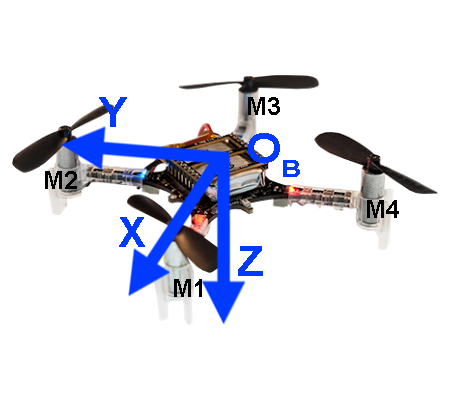
\includegraphics[width=.4\textwidth]{Images/frameBody}\label{fig:frameBody}}
\hspace{0.5cm}
\subfloat[Body frame in $\times$ configuration]{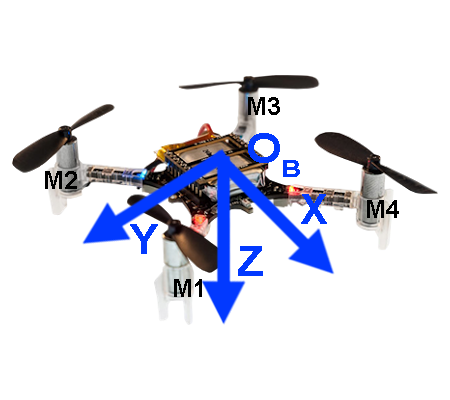
\includegraphics[width=.4\textwidth]{Images/frameBodyX}\label{fig:frameBodyX}}
\caption{Body frames in the two main configurations}
\label{fig:frames}
\end{figure}
  
Dynamics can be explained using a 12-variables state description of the Crazyflie with the following state vector: the position of $O_B$ with respect to the world-frame, the speed of $O_B$ with respect to the world-frame and  the attitude angles (Euler angles) and the angular speed in the body frame:
 \[\boldsymbol{x} =  [x \ y \ z \ \dot x \ \dot y \ \dot z \ \phi \ \theta \ \psi \ \omega_{xB} \ \omega_{yB} \ \omega_{zB}]^T \]

When the Crazyflie is at the origin of the world frame, without flying and the axes of both frames are aligned, the state is:
 \[\boldsymbol{x} =  [0 \ 0 \ 0 \ 0 \ 0 \ 0 \ 0 \ 0 \ 0 \ 0 \ 0 \ 0 ]^T\]
 
This is a simple model considering translations and rotations along three axes. Some more advanced models can also include also the accelerometers biases, the gyroscopes drift, or noise on the estimates, making easily a 20-or-more-states description of a drone. But this is behind the scope of this project.

\subsubsection{Attitude Representation}
The attitude can be defined as the relative orientation of the body-frame with reference to the world frame and, nowadays, several representations of the attitude  an object in space \cite{Diebel2006}. Among these representations, Euler angles, rotation matrices and unit quaternions are the most used. To derive the dynamics equations, we require the first two and the last one is implemented in the firmware for attitude estimation.

As stated above, the state of the drone includes its attitude in terms of Euler angles. The angles are the values of three ordered rotations around three axes in space and the sequence of the three axes around which, each rotation is accomplished, defines the sub-representation.  Officially, there is 12 valid sub-representations but two are considered as the main ones: the $(3,1,3)$ sequence and the $(1,2,3)$ sequence.

The first one, also known as the \emph{x-convention}, is often used in the study of spinning objects. The angles are called, in order, \emph{spin}, \emph{nutation} and \emph{precession}.

The second one, commonly found in aerospace engineering and computer graphics, is also often called \emph{Cardan angles}, \emph{Tait-Bryan angles} or \emph{nautical angles}. In this sub-representation, angles are called often as follow \emph{bank}, \emph{attitude}, \emph{heading} or \emph{roll}, \emph{pitch}, \emph{yaw}. 

From now on, referring to Euler angles refers to the latter sub-representation. Moreover, the roll-pitch-yaw convention for angles name is preferred.

Euler angles are defined as a sequence of three rotation to map the body-frame on the world-frame or inversely. For this purpose, first a rotation around the X-axis gives the roll angle $\phi$ , then a rotation around the Y-axis gives the pitch angle $\theta$ and finally a rotation around the the Z-axis gives the yaw angle $\psi$. The order $(X,Y,Z)$ is what gives this sub-representation its name $(1,2,3)$. On the figure~\ref{fig:attitude}, the roll angle corresponds to the rotation between the x''y''z'' and x'y'z' frames, the pitch x'''y'''z''' and x''y''z'' and the yaw xyz and x'''y'''z'''.
\[\boldsymbol{q} =  \begin{bmatrix} \phi \\ \theta \\ \psi \end{bmatrix}\]

Although, Euler angles are easy to visualize, they suffer from singularities. In the case of a pitch angle $\theta=90\degree$, variation in yaw angle are indistinguishable from variation in roll angle. However, these are extreme cases that are never met in the scope of this project.

\begin{figure}[htbp]
\centering
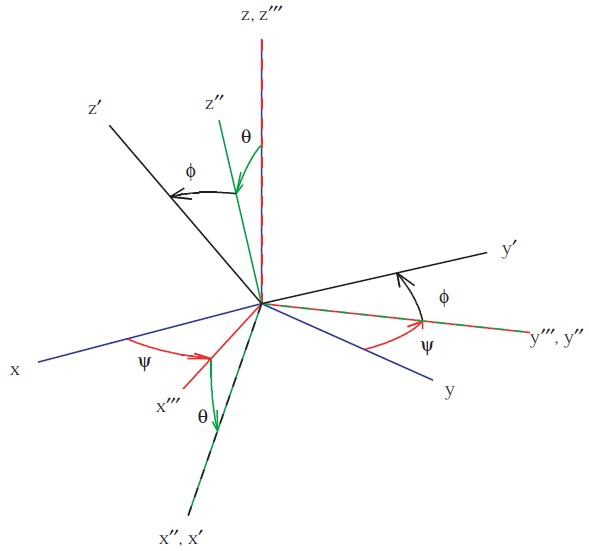
\includegraphics[width=0.5\textwidth]{Images/attitude}
\captionsetup[subfloat]{labelformat=empty}
\subfloat[Drawing from \cite{Diebel2006}]{\hspace{\linewidth}}
\caption{Roll $\phi$, Pitch $\theta$ and Yaw $\psi$ Angles}
\label{fig:attitude}
\end{figure}

The second convention for representing attitude is a rotation matrix. A rotation matrix maps a vector from the body frame to the world frame (or reversely) in a length-preserving manner. The reverse operation can be easily computed, as the all the matrix rotations are part of the special orthogonal group, their inverse is also their transpose.
\[ \boldsymbol{v_B} = R_{BW} \boldsymbol{v_W}\]
\[ \boldsymbol{v_W} = R_{WB} \boldsymbol{v_B}\]
\[ R_{BW} = R_{WB}^{-1} = R_{BW}^T \]

Each rotation in a 3-dimensional space can be decomposed in three rotations around the three main axes:
\[R_{Ox}(\alpha)  = \begin{bmatrix} 1 & 0 & 0 \\ 0 & \cos{\alpha} & -\sin{\alpha} \\ 0 & \sin{\alpha} & \cos{\alpha}  \end{bmatrix} R_{Oy}(\beta)  = \begin{bmatrix} \cos{\beta} & 0 & \sin{\beta} \\ 0 & 1 & 0 \\ -\sin{\beta} & 0 & \cos{\beta}  \end{bmatrix} R_{Oz}(\gamma)  = \begin{bmatrix} \cos{\gamma} & -\sin{\gamma} & 0 \\ \sin{\gamma} & \cos{\gamma} & 0 \\ 0 & 0 & 1  \end{bmatrix} \]

Consecutive rotations can be easily combined by left-multiplying the matrices. Although its simplicity, the representation uses requires 9-states variable. Therefore, Euler angles are kept for representation and a transition to rotation matrix is performed for computation purposes.

The mapping between Euler angles and rotation matrix, consisting of the multiplication of the three individual rotation matrices in the right order, and is computed as follow ($c_\alpha$ corresponds to $\cos{\alpha}$ and $s_\alpha$ to $\sin{\alpha}$):
\[R_{BW}(\phi, \theta, \psi)= R_{Ox}(\phi) R_{Oy}(\theta) R_{Oz}(\psi)  = 
\begin{bmatrix}  c_\theta c_\psi  & c_\theta s_\psi  & -s_\theta  \\ s_\phi s_\theta c_\psi -c_\phi s_\psi  & s_\phi s_\theta s_\psi  + c_\phi c_\psi  & c_\theta s_\phi  \\ c_\phi s_\theta c_\psi +s_\phi s_\psi  & c_\phi s_\theta s_\psi -s_\phi c_\psi  & c_\theta c_\phi  \end{bmatrix} \]

Finally the last convention is the unit quaternion. The unit quaternion is a 4-dimensional generalization of complex numbers whose norm $\norm{\boldsymbol{q}} = 1$.
\[ \boldsymbol{q} =  q_0 + q_1 \cdot i + q_2 \cdot j + q_3 \cdot k = \begin{bmatrix} q_0 \\ q_1 \\ q_2 \\ q_3 \end{bmatrix} = \begin{bmatrix} q_0 \\ q_{1:3} \end{bmatrix} \]

They profit from most of the tools of complex algebra such:
\[ \boldsymbol{\bar q} = \begin{bmatrix} q_0 \\ -\boldsymbol{q}_{1:3} \end{bmatrix},  \quad \norm{\boldsymbol{q}} = \sqrt{q_0^2 + q_2^2 + q_3^2 + q_4^2}, \quad \boldsymbol{q}^{-1} = \frac{\boldsymbol{\bar q}}{ \norm{\boldsymbol{q}}} \]

However, multiplication is non-commutative:
\[\boldsymbol{q} \cdot \boldsymbol{p} = \begin{bmatrix} q_0p_0 - \boldsymbol{q}^T_{1:3}\boldsymbol{p}_{1:3} \\ q_0\boldsymbol{p}_{1:3} + p_0\boldsymbol{q}_{1:3} - \boldsymbol{q}_{1:3} \times \boldsymbol{p}_{1:3} \end{bmatrix} \]

Equivalently, a vector in the world frame can be mapped in the body frame:
\[ \begin{bmatrix} 0 \\ \boldsymbol{v_B} \end{bmatrix}  = \boldsymbol{q} \cdot \begin{bmatrix} 0 \\ \boldsymbol{v_W} \end{bmatrix} \cdot \boldsymbol{q}^{-1} \]

The attitude estimation on the CrazyFlie is computed using quaternions and then mapped into Euler angles for control. A detailed explanation can be found in appendix ~\ref{app:att_estim}.

The weakness of unit quaternions is, especially in optimization problem like MPC, enforcing the quadratic constraints on the norm. Although several methods exist to solve this problem, none of them is satisfying enough.
\subsection{Newton-Euler equations}
\label{sec:dynamicsEquations}

\begin{figure}[htbp]
\centering
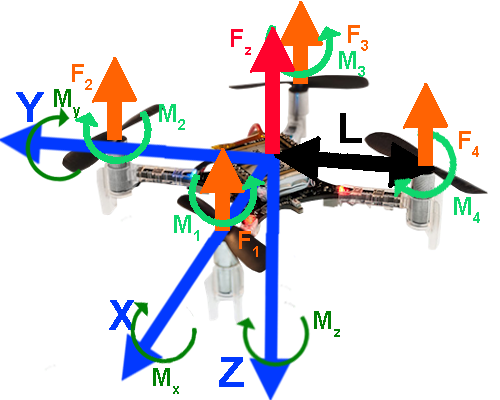
\includegraphics[width=0.5\textwidth]{Images/forceMoments}
\caption{Force and torques applied on the CrazyFlie}
\label{fig:forceMoment}
\end{figure}

In a quadcopter, each propeller generates a force $F_i$ and a torque $M_i$ proportional to the square of its spinning speed  (c.f.: figure~\ref{fig:forceMoment}). The vector $\boldsymbol{u}$ is the vector of the squared spinning rates.
\[ \boldsymbol{u} = [\omega^2_1 \  \omega^2_2 \  \omega^2_3 \  \omega^2_4]^T \]
\[F_i =  K_f  u_i \ \ \ M_i = K_f  u_i  ,\  i = 1,2,3,4\]

In a ''\emph{plus}'' configuration, the thrust force (or simply thrust) $F_{z}$ and the torques $M_{x}, M_{y}, M_{z}$  applied to the center of mass of the quadrotor, depends on $\boldsymbol{u}$:
\[  
\begin{bmatrix}
F_{z}\\ 
M_{x}\\
M_{y}\\
M_{z}
 \end{bmatrix}_B
=
\begin{bmatrix}
K_f & K_f & K_f & K_f\\
0 & -K_f \cdot L & 0 & K_f \cdot L\\
K_f \cdot L & 0 & -K_f \cdot L & 0\\
-K_t & K_t & -K_t & K_t
\end{bmatrix}
\textbf{u} = K\textbf{u}
\]
Where $L$ is the distance from the axis of rotation of a motor and $O_b$.

The dynamics of a quadrotor can now be derived using Newton-Euler equations:
\[ m\boldsymbol{\ddot r} =  \sum_i \boldsymbol{F_i} = \boldsymbol{G} + \boldsymbol{T} + \boldsymbol{D} = \begin{bmatrix}  0\\ 0\\ mg \end{bmatrix} + R_{BW}^T(\phi, \theta, \psi) \begin{bmatrix}  0\\ 0\\ -F_z \end{bmatrix}_B + \begin{bmatrix}  D_x\\ Dy\\ D_z \end{bmatrix}\]
\[ I\boldsymbol{\dot \omega_B} =  \sum \boldsymbol{M_B} - \boldsymbol{\omega_B}  \times (I \boldsymbol{\omega_B} )=  
\begin{bmatrix}  M_{x}\\ M_{y}\\ M_{z} \end{bmatrix}_B - \boldsymbol{\omega_B}  \times (I \boldsymbol{\omega_B}) \]
Where $\boldsymbol{r}$ is the position of $O_B$, expressed in the world frame,  $\boldsymbol{G}$ is the gravity force, $\boldsymbol{T}$ is the thrust force generated by the propellers, $\boldsymbol{D}$ is the drag force, $I$  is the inertia matrix of the quadcopter and $\boldsymbol{\omega_B}$ is the angular speed in the body frame.

To fully define the quadrotor, the attitude rates to body rate matrix $W(\phi,\theta,\psi)$ is still required: %Note for me: In reference document, the matrix is [E']^{-1}
\[ W(\phi,\theta,\psi) = \begin{bmatrix}  1 & \sin\phi \tan\theta  & \cos\phi \tan\theta \\ 0 & \cos\phi  &-\sin\phi  \\ 0 & \frac{\sin\phi }{\cos\theta } & \frac{\cos\phi }{\cos\theta } \end{bmatrix}\]
\[ \boldsymbol{ \dot q} = \begin{bmatrix} \dot \phi \\ \dot \theta\\ \dot \psi \end{bmatrix} = W(\phi,\theta,\psi) \boldsymbol{\omega_B}\]

\subsection{Full model}
 \[\boldsymbol{x} =  [x \ y \ z \ \dot x \ \dot y \ \dot z \ \phi \ \theta \ \psi \ \omega_{xB} \ \omega_{yB} \ \omega_{zB}]^T \]
 \[ \boldsymbol{u} = [\omega^2_1 \  \omega^2_2 \  \omega^2_3 \  \omega^2_4]^T \]
\[\left\{ \begin{matrix}[l]
\begin{bmatrix} \dot x_{1}\\\dot x_{2} \\ \dot x_{3} \end{bmatrix} = \begin{bmatrix}  x_{4}\\ x_{5} \\ x_{6} \end{bmatrix}\\
\begin{bmatrix} \dot x_{4}\\\dot x_{5} \\ \dot x_{5} \end{bmatrix} = \frac{1}{m}(\begin{bmatrix}  0\\ 0\\ -mg \end{bmatrix} + R_{BW}^T(x_7, x_8, x_9) \begin{bmatrix}  0\\ 0\\ F_{z}(\boldsymbol{u}) \end{bmatrix}_B + (\begin{bmatrix}  D_x\\ D_y\\ D_z \end{bmatrix})\\
\begin{bmatrix} \dot x_{7}\\\dot x_{8} \\ \dot x_{9} \end{bmatrix} = W(x_7, x_8, x_9)\begin{bmatrix}  x_{10}\\ x_{11} \\ x_{12} \end{bmatrix} \\
\begin{bmatrix} \dot x_{10}\\\dot x_{11} \\ \dot x_{12} \end{bmatrix} = I^{-1}(\begin{bmatrix}  M_{x}(\boldsymbol{u})\\ M_{y}(\boldsymbol{u})\\ M_{z}(\boldsymbol{u}) \end{bmatrix}_B - \begin{bmatrix}  x_{10}\\ x_{11} \\ x_{12} \end{bmatrix} \times (I\begin{bmatrix}  x_{10}\\ x_{11} \\ x_{12} \end{bmatrix}))\\
\end{matrix} \right.\]

\newpage
\section{High-Level Control - Formation Control}
Collective movement is widely observed phenomenon in the wild and civilized worlds. In animal societies, the phenomenon, called flocking, herding, schooling or swarming, depending on the species, happens for all size of groups, for all size of individuals, homo- or heterogeneous groups and sometimes can be circumstance-driven, like migrations. A flock, generally used to describe any of the denomination introduced before, is characterized by directed movement and quick reactions to obstacle at the global scale, even though there is no leader. Among the benefits of group motion, dilution of risk, improved exploration, foraging and sensing capabilities, energy saving are the most interesting. Of course costs arise also from group formation like the diminution of resource per capita but these concern mostly living entities \cite{Krause2002, Parrish1997}.

Flocks of robots are a perfect example of swarm or distributed intelligence, in which global structure appears solely through numerous local interactions \cite{Bonabeau1999, Reynolds1987}. Indeed, computing trajectories for every robots, taking into account other robots, obstacles and some other constraints can soon become intractable when the number of robots increase. For collective motion in robotics, however, another kind of collective movement exists, motion in formation. Compared to flocking, where the relative location and the neighborhood of an individual is in permanent evolution, motion in formation assigns a specific position to each member and its neighborhood becomes static. Despite these constraints, this collective motion can also be implemented using a distributed control architecture, knowing that each individual needs to be assign a specific position in the formation. While flocking benefits more from robustness, flexibility and scalability, formations are more efficient, require less individuals for an equivalent coverage and are more intuitively commanded. Of course, the ideal group configuration depends on the application, the environment and the type of robot. Concerning this work, it will focus on motion in formation.\\
In a more global point of view, swarm robotics, compared to a single robot achieving the identical task, require simpler units and increase reliability \cite{Beni2004}. The former implies simpler hardware, software, as well as sensing, acting and communicating capabilities. But, often in distributed intelligence, the cost of robustness is efficiency, in terms of time, total energy required or eventually another metrics. Or, restated, swarm robotics needs to carefully balance exploration et exploitation behaviors.

\subsection{Taxonomy}
When studying formations, the taxonomy defined in \cite{Arkin1999} about position determination serves as reference. In each possibility, each robot compute its place in the formation with respect to a given physical or mathematical landmark.
\begin{itemize}
\item \emph{Unit-centered formation}. The unit center of a formation corresponds to its center of mass. While, this position determination configuration seems to achieve the best results, it can often be inadequate given the application. Moreover in case of fully distributed control, it requires a global knowledge of the position of every member of the formation, which can be implemented through communication channels or sufficiently performing sensing capabilities.
\item \emph{Leader-referenced formation}. The reference is one of the member of the group, the leader. This configuration achieves also good results and is ideal when the leader is human-controlled. However, it is constantly necessary to know, or being able to measure, the (relative) position of the leader, which can require either a long range-communication, or sensing module, depending on the application and the localization method.
\item \emph{Neighbor-referenced formation}. In this case, there is no common reference. Each member of the formation determines its position from the position of a unique other member. Although it is more demanding in terms of emitters than a leader referenced formation, the range of communication can be considerably reduced. In case of relative localization without communication, this configuration has the lowest requirements in term of range. Note also that mixed leader-neighbor referenced formations can exist \cite{Mataric2002}. This is suitable when one leader is human-controlled and the individuals have low-range communication capabilities.
\end{itemize}

\subsection{Implementation}
Formation control can be implemented in various ways but we will focus on two, already widely implemented, from behavior-based control \cite{Arkin1999, Mataric2002, Pugh2009} to graph-based control  \cite{Gowal2013, Falconi2010}. Both of these methods can easily be implemented in a distributed system for any of the configuration presented previously using relative localization sensors and IDs. But before selecting one of these methods, constraints of the actual control architecture have to be considered required. Indeed the MPC position controller can takes specific input vectors. Therefore, if a formation control block is devised, it can take as many input as wanted but the output must necessarily be a 6-state vector of three positions and three velocities for each drone.

Behavioral controllers, used in the form of motor-schema or, also called, potential field methods \cite{Arkin1999, Pugh2009} is an elegant way for designing adaptive controllers. Several zone can be defined, in which the potential can be chosen freely in order to induce the desired reaction. Typically the potential provides a speed vector from which position can be integrated. This approach can be implemented for any type of formation. An example of three-zones potential could be the following:
\[ \dot r_i =  \left\{ \begin{matrix*}[l] 0 & if\ r_{f,i}-r_i\ \in [0; d_1] \\ \alpha(r_{f,i}-r_i-d_1) & if\ r_{f,i}-r_i\ \in [d_1; d_2] \\  \beta(r_{f,i}-r_i-d_2)^2 + \alpha(r_{f,i}-r_i-d_1) & if\ r_{f,i}-r_i\ \in [d_2; \inf] \end{matrix*} \right. \ for\ i = 1,2,3\]
Where $r_{f,i}$ is the reference position in formation, $r_i$ the current position in one dimension, $d_1$, $d_2$, $\alpha$ and $\beta$ are parameters

\begin{figure}[htbp]
\centering
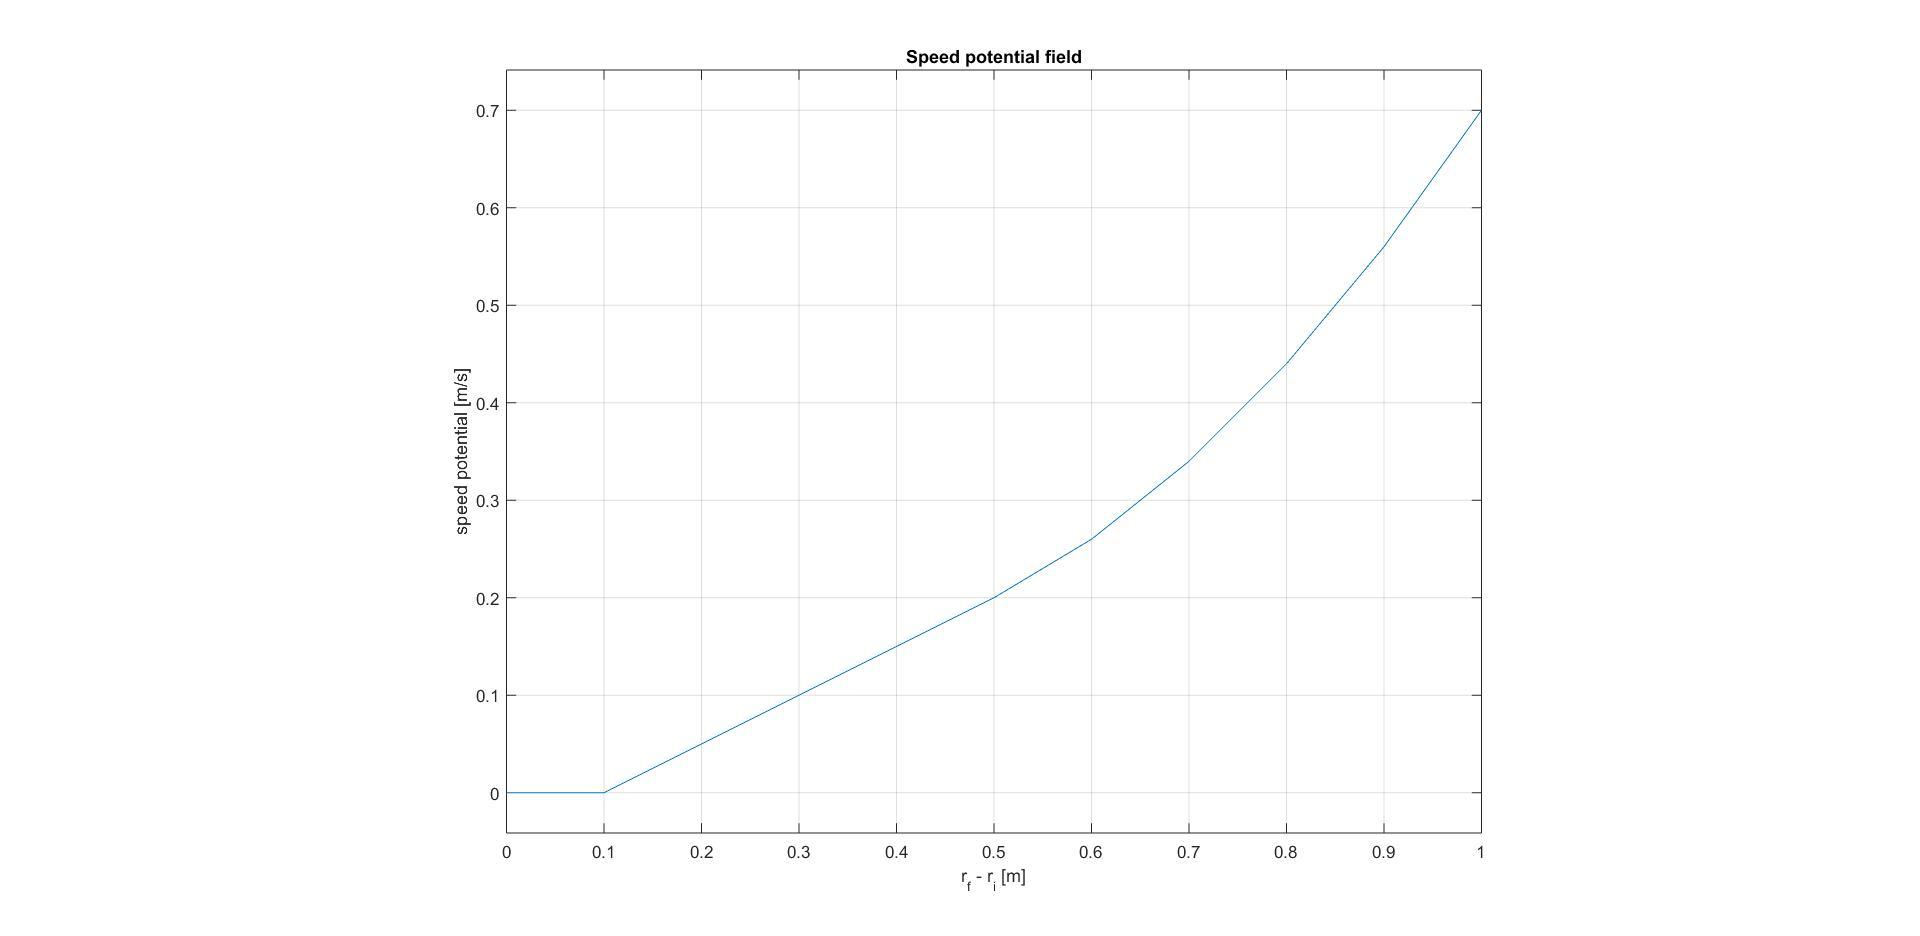
\includegraphics[width=.8\textwidth]{Images/potentialEx}
\caption{An example of attractive potential field}
\label{fig:potentialEx}
\end{figure}

Graph-based control seems well adapted to provide a reference vector for leader- or neighbor-referenced formations. This kind of controllers are derived from so-called consensus problems, which try to make a set of agent with different initial states converge to a single final state, identical for all agents. \cite{Ren2005}. The Rendez-vous problem \cite{Gowal2013} is one of these problems perfectly adapted to formation control. Required notions of graph theory are: 
\begin{itemize}
\item $\mathcal{G} = <\mathcal{N}, \mathcal{E}>$, an (un)directed graph.
\item $\mathcal{N} = \{R_1, \cdots, R_n\}$, the finite nodes set,  with $n$, the number of robots.
\item $\mathcal{E} \in \mathcal{N}^2, \mathcal{E} = \{(Ri,Rj)| R_i, R_j \in \mathcal{N} and\ i \neq j\} = \{e_1, \cdots, e_m\} $, the (un)directed finite edges set.
\item $A \in  \mathbb{R}^{n \times n} $, the adjacency matrix is a symmetric matrix, the image of the connections between the nodes:
\[a_{ij} =  \left\{ \begin{matrix*}[l] 1 & if\ (R_i, R_j)\ or\ (R_j, R_i) \in \mathcal{E} \\ 0 & else \end{matrix*} \right.\]
\item $D \in  \mathbb{R}^{n \times n} $, the degree matrix is a symmetric matrix, whose diagonal elements represent the cardinality of each node (i.e.: the sum of edges originating or arriving in this node):
\[d_{ii} =  \sum_{j=1}^{N} a_{ij}\]
\item $B \in  \mathbb{R}^{n \times m} $, the incidence matrix is a matrix, describe which node is connected using which edge. In undirected graphs, edge are given a random direction.
\[b_{ij} =  \left\{ \begin{matrix*}[l] 1 & if\ e_j = (R_i, \bullet) \\-1 & if\ e_j = (\bullet, R_i)  \\ 0 & else \end{matrix*} \right.\]
\item $W \in \mathbb{R}^{m\times m} $, a diagonal weight matrix whose element $w_{i,i}$ corresponds to the weight of edge $e_i \in \mathbb{E}$.
\item $L$ and $L_w\in \mathbb{R}^{n\times n} $, the Laplacian and the weighted Laplacian matrices:
\[ L = D-A = BB^T \qquad L_w = BWB^T\]
\end{itemize}  
The Laplacian and the weighted Laplacian matrices benefits from interesting properties: They positive-semidefinite. This implies that all eigenvalues are nonnegative. Moreover, at least one eigenvalue isequal to zero. Proofs can be found in \cite{Gowal2013}. 

The feedback law, for state $i$ of all nodes in a N-state system is:
\[ \boldsymbol{\dot x_i}(t) = - L\boldsymbol{x_i}(t)\ for\ i=1, \cdots, N \]
\[\boldsymbol{x_i}(t) \in \mathbb{R}^n\]
Below, in figure~\ref{fig:graphs}, we show the directed graph for the leader-referenced formation and one possible graph for a neighbor-referenced formation. we will quickly compute the matrices $A$, $D$, $B$ and $L$. We assume $W = I_{n}$, however in the neighbor-referenced case, it could be a good interesting to increase the weight of the edges $(R_1, R_3)$ and $(R_3, R_1)$, as they are central to the formation directed graph.

\begin{figure}[h]
\centering
\subfloat[The leader-referenced graph]{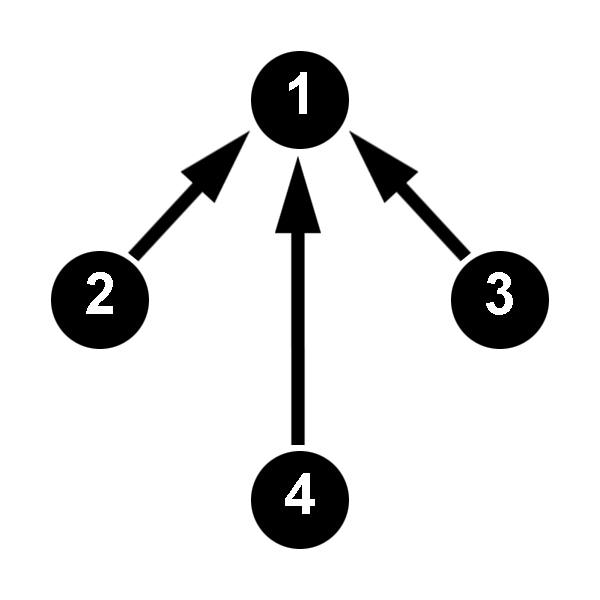
\includegraphics[width=.4\textwidth]{Images/graphLeader}\label{fig:graphLeader}}
\hspace{0.5cm}
\subfloat[A neighbor referenced graph]{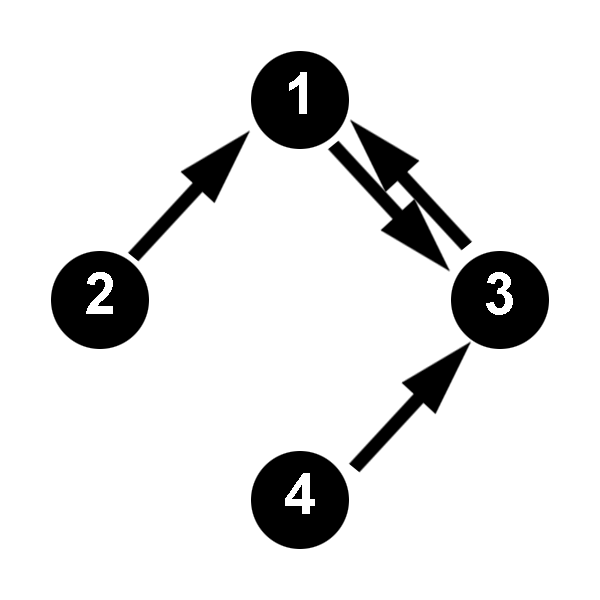
\includegraphics[width=.4\textwidth]{Images/graphNeighbor}\label{fig:graphNeighbor}}
\caption{The directed graphs for a leader-referenced formation and a neighbor-referenced}
\label{fig:graphs}
\end{figure}

\begin{displaymath}
\begin{aligned}
A_{leader} &= \begin{bmatrix} 0 & 1 & 1 & 1 \\ 1 & 0 & 0 & 0 \\ 1 & 0 & 0 & 0 \\ 1 & 0 & 0 & 0\end{bmatrix} 		& A_{neighbor} &= \begin{bmatrix} 0 & 1 & 1 & 0 \\ 1 & 0 & 0 & 0 \\ 1 & 0 & 0 & 1 \\ 0 & 0 & 1 & 0\end{bmatrix} \\
D_{leader} &= \begin{bmatrix} 3 & 0 & 0 & 0 \\ 0 & 1 & 0 & 0 \\ 0 & 0 & 1 & 0 \\ 0 & 0 & 0 & 1\end{bmatrix}		& D_{neighbor} &= \begin{bmatrix} 3 & 0 & 0 & 0 \\ 0 & 1 & 0 & 0 \\ 0 & 0 & 3 & 0 \\ 0 & 0 & 0 & 1\end{bmatrix} \\
B_{leader} &= \begin{bmatrix} -1 & -1 & -1 \\ 1 & 0 & 0 \\ 0 & 1 & 0 \\ 0 & 0 & 1\end{bmatrix} 				& B_{neighbor} &= \begin{bmatrix} 1 & -1 & -1 & 0 \\ 0 & 1 & 0 & 0 \\ -1 & 0 & 1 & -1 \\ 0 & 0 & 0 & 1\end{bmatrix} \\
L_{leader} &= \begin{bmatrix} 3 & -1 & -1 & -1 \\ -1 & 1 & 0 & 0 \\ -1 & 0 & 1 & 0 \\ -1 & 0 & 0 & 1\end{bmatrix} 	& L_{neighbor} &= \begin{bmatrix} 3 & -1 & -2 & 0 \\ -1 & 1 & 0 & 0 \\ -2 & 0 & 3 & -1 \\ 0 & 0 & -1 & 1\end{bmatrix}
\end{aligned}
\end{displaymath}

The discrete equivalent of the Laplacian feedback control requires another matrix \cite{Moreau2005}, $L_k \in \mathbb{R}^{n \times n}$, the stochastic weight of links matrix. In a stochastic matrix, the sum of every row is equal to one. Therefore, 1 is an eigenvalue and $\boldsymbol{1}_n$ is the corresponding eigenvector.
\[l_{ij} =  \left\{ \begin{matrix*}[l] \omega_{ij} > 0 & if\  = (R_i, R_j) \in \mathbb{E}\ or\ i=j\\ 0 & else \end{matrix*} \right.\]

The feedback law become, for state $i$ of all nodes in a N-state system:
\[ \boldsymbol{x_i}(k+1) = L_k\boldsymbol{x_i}(k)\ for\ i=1, \cdots, N \]
\[\boldsymbol{x_i}(t) \in \mathbb{R}^n\]

Again for the graphs in figure~\ref{fig:graphs}, assuming a equal weight for all edges, we provide the discrete equivalent of the Laplacian matrix:
\begin{displaymath}
\begin{aligned}
L_{k,leader} &= \begin{bmatrix} 1 & 0 & 0 & 0 \\ \frac{1}{2} & \frac{1}{2} & 0 & 0 \\ \frac{1}{2} & 0 & \frac{1}{2} & 0 \\ \frac{1}{2} & 0 & 0 & \frac{1}{2}\end{bmatrix} 		& L_{k,neighbor} &= \begin{bmatrix} \frac{1}{2} & 0 & \frac{1}{2} & 0 \\ \frac{1}{2} & \frac{1}{2} & 0 & 0 \\ \frac{1}{2} & 0 & \frac{1}{2} & 0 \\ 0 & 0 & \frac{1}{2} & \frac{1}{2}\end{bmatrix} \\
\end{aligned}
\end{displaymath}

Another control method can be devised, taking the control architecture into account. It consists of directly acting on the MPC controller constraints or objective function\textcolor{red}{[CITATIONS]}.  By implementing formation control in such a way, no additional block needs to be integrated in the current architecture. However, a more in-depth work in the controller is required as, an ideal formulation of cost and a weight need to be found. Moreover this approach reduce the modularity of the control system in its global aspect.

\subsection{Measuring stability}
\cite{Mataric2002}
\begin{itemize}
\item distance on formation line.
\item distance perpendicular to formation line.
\item angle deviation.
\end{itemize}

\subsection{Measuring robustness}

\subsection{Evaluation}
\begin{itemize}
\item time to formation (static ref) tToForm\_refStatic.
\item time to formation (dynamic ref) tToForm\_refDynamic.
\item \% time in formation (normalized by (tTot-tToForm).
\item average deviation from formation position (after tToForm).
\item max deviation from formation position (after tToForm).

\end{itemize}

\cite{Arkin1999}
\cite{Mataric2002}

\newpage
\section{Low-Level Control}
\subsection{Control Architecture}
\subsection{Inner Controller}
\label{sec:innerControl}
The inner controller, responsible for attitude control can be found in the stabilizer.c module. Its main loop can be divided in four steps, the corresponding file are indicated in brackets:
\begin{itemize}
\item State acquisition (\emph{sensors\_stock.c} and \emph{estimator\_complementary.c}  or \emph{estimator\_kalman.c}).
\item Reference acquisition (\emph{commander.c}).
\item Control step (\emph{controller\_pid.c} and then \emph{attitude\_pid\_controller.c} and \emph{pid.c}).
\item Motor distribution (\emph{power\_distribution\_stock.c}).
\end{itemize}

\subsubsection{State and reference acquisition}
Independently of the chosen estimation method, 13-states Kalman filter or attitude update through Mahony or Magdwick quaternion method, the first step will provide data for attitude angles and rates. However, Kalman estimator allows the stabilizer loop to run only at 500 Hz, while the other method allows 1000 Hz. Sensor acquisition runs at 500 Hz for IMU and 100 Hz for barometer. In the second estimaiton method, attitude is updated at 250 Hz and position (if wanted) at 100 Hz. For Kalman, update are performed at 100 Hz for all state, barometer is processed at 25 Hz.

During the acquisition of the references, the inner control architecture is also defined or updated. Depending on the control mode, the reference are translated differently and the chain of controller is activated accordingly. There are six configuration variables, each can be set in absolute, velocity or disabled mode.  These variables are X, Y, Z, the 3D positions and roll, pitch, yaw, the three attitude angles. For this project, the configuration implies that the reference are always going to be roll angle, pitch angle, yaw rate and thrust (c.f.: table~\ref{tab:setpointConfig}). Despite the presence of a magnetometer in the IMU, it is not yet integrated in the firmware, therefore an absolute yaw positioning is not possible.
\begin{table}[h]
\centering
\caption{Reference and inner control architecture configuration}
\begin{tabular}{|l|c|}
\hline
\textbf{Configuration variables} & \textbf{State}  \\
\hhline{|=|=|}
Position X & Disabled \\
\hline
Position Y & Disabled \\
\hline
Position Z & Disabled \\
\hline
Attitude Roll & Absolute\\
\hline
Attitude Pitch & Absolute\\
\hline
Attitude Yaw & Velocity\\
\hline
\end{tabular}
\label{tab:setpointConfig}
\end{table}

\subsubsection{Controllers}
The first module, \emph{controller\_pid.c}, defines the control architecture and the rate of the two sub-control loops: PID at 100 Hz for position control or cascade controllers at 500 Hz for attitude control. In the latter (\emph{attitude\_pid\_controller.c}), the yaw rate reference is first integrated to obtain a yaw reference angle, then, the first layer of control is given the attitude angles references and estimations. In the second layer, rates are controlled. The output of the attitude controllers serve as rate reference and the gyros as attitude rate as measurement (c.f.: figure~\ref{fig:controllerCascade}). This assumption can be considered as true for small angles or first-order approximations. For exact attitude rate computation, refer to the section~ref:{sec:dynamicsEquations}.  In the cascade controller, both layers  are composed of standard PID controllers using an integral limit as shown in figure~\ref{fig:controllerPID}. Note also that the estimation method has an influence on the gains. In table~\ref{tab:controllerInnerGains}, gains are provided for a CrazyFlie 2.0 using the stock estimator.

\begin{figure}[h]
\centering
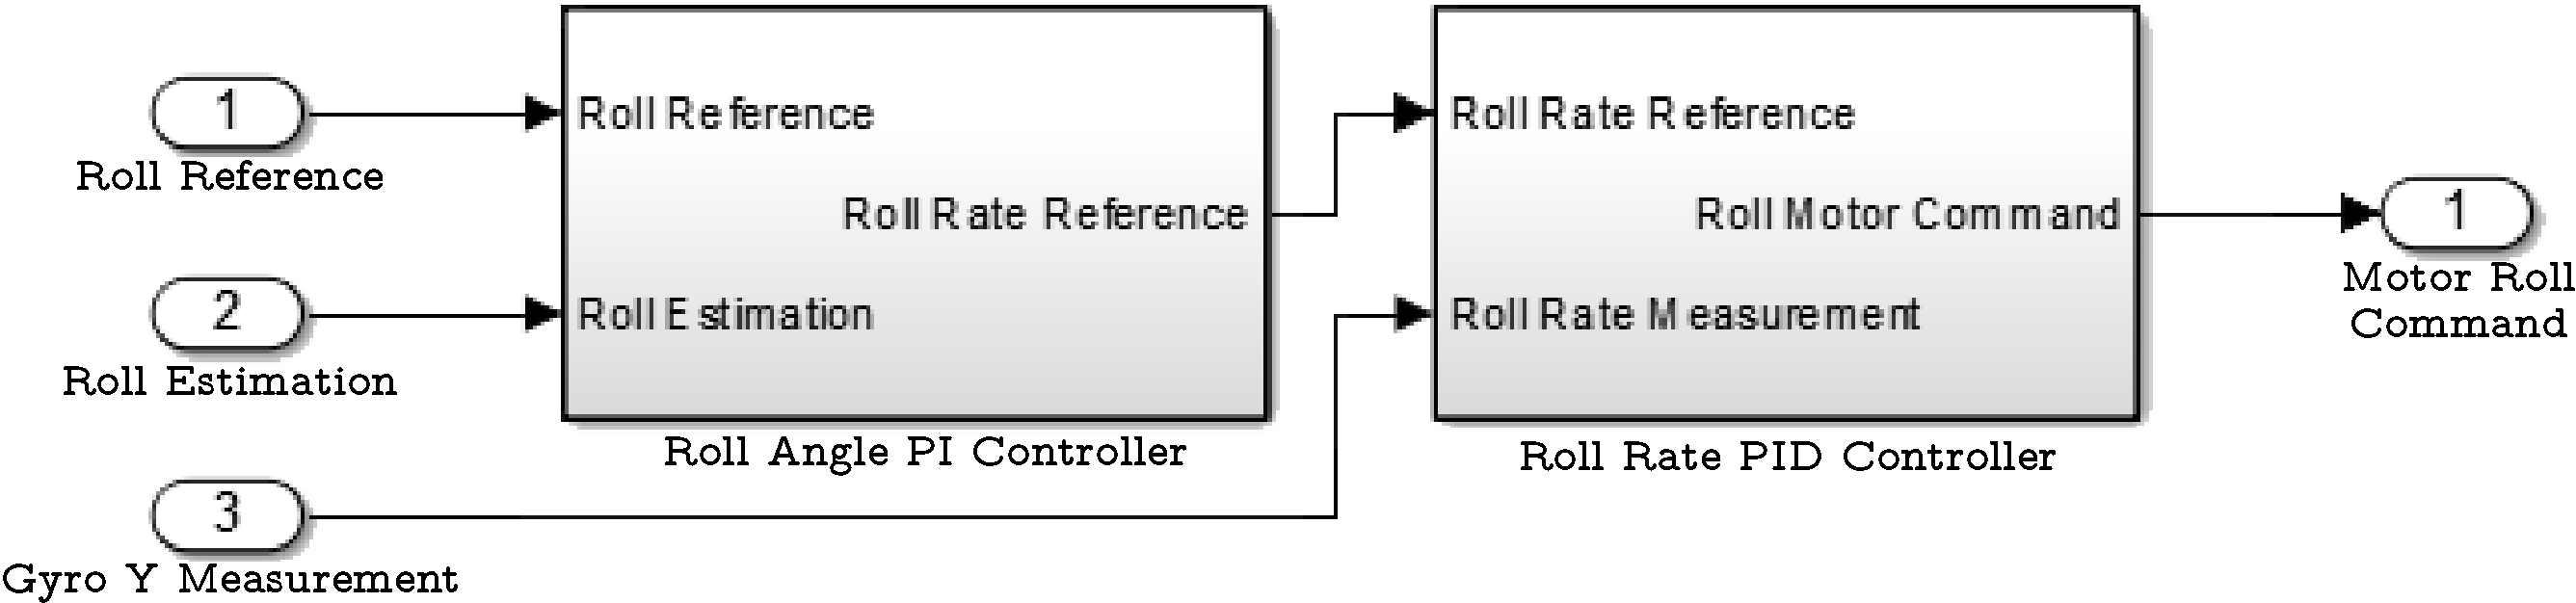
\includegraphics[scale = 0.8]{Images/controllerCascade}
\caption{Roll cascade controller architecture}
\label{fig:controllerCascade}
\end{figure}

\begin{figure}[h]
\centering
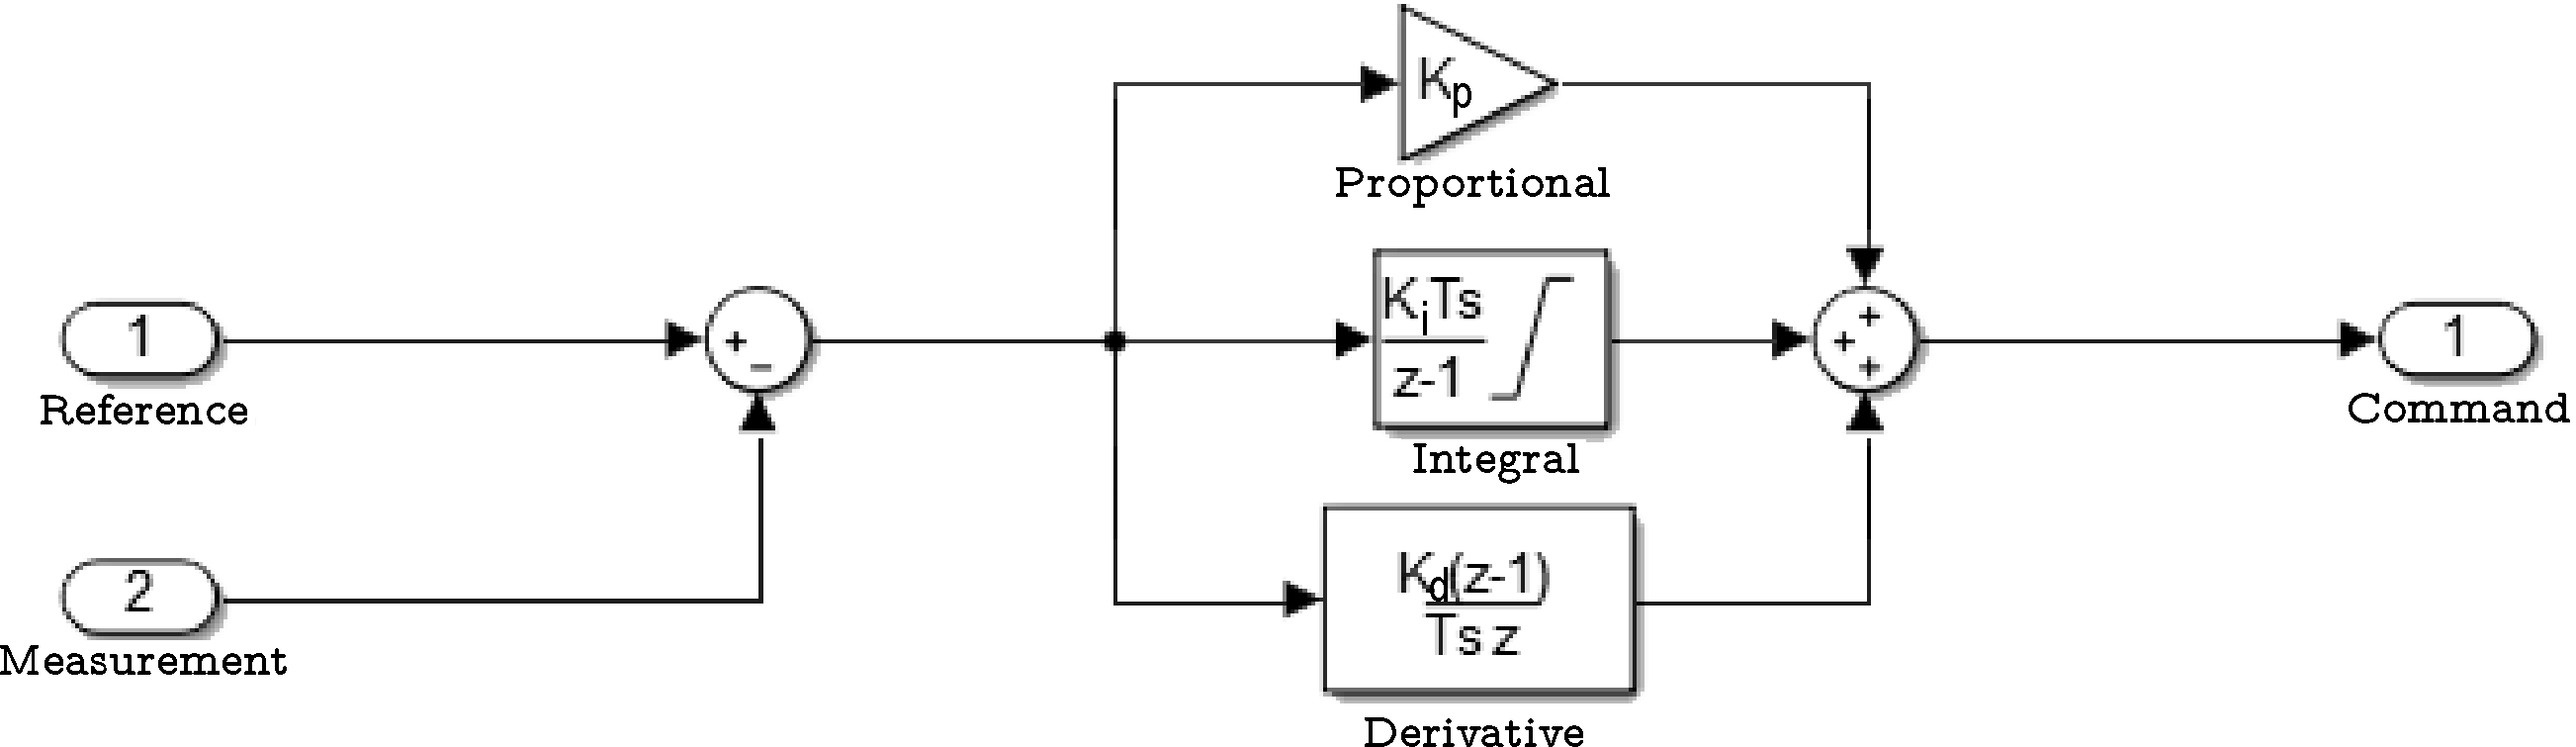
\includegraphics[scale = 0.8]{Images/controllerPID}
\caption{PID controller architecture}
\label{fig:controllerPID}
\end{figure}

\begin{table}[htdp]
\caption{Gains and integral limit of the inner PID controllers}
\centering
\begin{tabular}{|l||c|c|c|c|}
\hline
\textbf{Controller} & $\boldsymbol{K_p}$ & $\boldsymbol{K_i}$ & $\boldsymbol{K_d}$ & \textbf{Integral Limit}  \\
\hhline{|=#=|=|=|=|}
Roll & 6 & 3 & 0 & 20  \\
\hline
Pitch & 6 & 3 & 0 & 20  \\
\hline
Yaw & 6 & 1 & 0.35 & 360  \\
\hline
Roll rate & 250 & 500 & 2.5 & 33.3  \\
\hline
Pitch rate & 250 & 500 & 2.5 & 33.3  \\
\hline
Yaw rate rate & 70 & 16.7 & 0 & 166.7  \\
\hline
\end{tabular}
\label{tab:controllerInnerGains}
\end{table}

\subsubsection{Motor distribution}
The output of the 3 attitude cascade controllers and the thrust input are combined, with respect to the flying configuration, as shown in table~\ref{tab:motorDistribution}, saturated and converted to a 8-bit value before being sent as PWM commands to the motors. 

\begin{table}[htdp]
\caption{Command summation for a $+$  flying configuration}
\centering
\begin{tabular}{|l|l c l c l|}
\hline
\textbf{Motor 1} & $u_{thrust}$ & + &$u_{pitch}$ & + & $u_{yaw}$\\
\hline
\hline
\textbf{Motor 2} & $u_{thrust}$ & - & $u_{roll}$ & - & $u_{yaw}$ \\
\hline
\hline
\textbf{Motor 3} & $u_{thrust}$ & - & $u_{pitch}$ & + & $u_{yaw}$\\
\hline
\hline
\textbf{Motor 4} & $u_{thrust}$ & + & $u_{roll}$ & - & $u_{yaw}$ \\
\hline
\end{tabular}
\label{tab:motorDistribution}
\end{table}

\subsection{Force to Angle and Thrust Commands}
\subsection{Outer Controller}

The outter posiiton controller is part of the receiding horizon controllers, or model prective controller, family. This type of controllers are well suited for constrained situations, strongly nonlinear systems or, as the name implies, for some future knowledge \cite{Borelli2015}. In a standard closed-loop implementation, the controller plans a series of $N$ discrete actions for the open-loop problem, corresponding to the following $N$ time steps. $N$ is called the horizon length. Because the model is often inacurate, or because the environment is evolving, after executing the first action command, the controller measures the state and/or its surrounding and re-plans a serie of $N$ actions acoordingly, which act as feedback. The longer the horizon length, the closer the prediction (the $N$ planned actions) from the closed-loop response. Despite it's power, MPC suffers from chalenges to attain: feasibility, stability, robustness and implementation. \textcolor{red}{A DEVELOPPER}.

\subsubsection{Implementation}
In optimization-based control, such as MPC, a necessary condition for optimal trajectory in a control system $\Sigma$ is the Pontryagin maximum principle \cite{Pontryagin1987, Lewis2006, Murray2010}. A control system is defined as follow, with $\mathcal{X} \subset \mathbb{R}^n$, the state set and $\mathcal{U} \subset \mathbb{R}^m$, the input set
\[ \Sigma = (\mathcal{X}, f, \mathcal{U}) \]
\[ \Sigma: \dot x = f(\boldsymbol{x}, \boldsymbol{u}),\ \boldsymbol{x} \in \mathcal{X},\ \boldsymbol{u} \in \mathcal{U} \]

Two important objects need to be presented, the Lagrangian $\mathcal{L}$ and the extended Hamiltonian $\mathcal{H}_{\Sigma,\mathcal{L}}$. The Lagrangian is a continuous function defined as follow, and subsequently used to define an objective function $J_{\Sigma,\mathcal{L}}$:
\[ \mathcal{L}: \mathcal{X} \times \bar{\mathcal{U}} \rightarrow \mathbb{R} \]
\[ \mathcal{L} := \mathcal{L}(\boldsymbol{x}, \boldsymbol{u}),\ \boldsymbol{x} \in \mathcal{X},\ \boldsymbol{u} \in \mathcal{U} \]
\[ J_{\Sigma,\mathcal{L}}: \mathcal{X} \times \mathcal{U} \times \mathbb{R_+} \rightarrow \mathbb{R} \]
\[ J_{\Sigma,\mathcal{L}}(\boldsymbol{\xi}, \boldsymbol{\mu}, t) = \int_{t}^{t+T} \mathcal{L}(\boldsymbol{\xi}(t), \boldsymbol{\mu}(t))dt, \ (\boldsymbol{\xi}(t), \boldsymbol{\mu}(t)) \in  \mathcal{X} \times \bar{\mathcal{U}}\]

The couple $(\boldsymbol{\xi}(t), \boldsymbol{\mu}(t))$ is called a trajectory.

In order to minimize  $J_{\Sigma,\mathcal{L}}$, three necessary conditions can be derived. However another mathematical object can be used, the extended Hamiltonian. It requires also the introduction of the co-state variable, or Lagrange multipliers $\boldsymbol{p}$:
\[ \mathcal{H}_{\Sigma,\mathcal{L}}: \mathcal{X} \times \mathcal{U} \times \mathbb{R}^n \rightarrow \mathbb{R} \]
\[ \mathcal{H}_{\Sigma,\mathcal{L}}(\boldsymbol{x}, \boldsymbol{u}, \boldsymbol{p}) = \boldsymbol{p}^Tf(\boldsymbol{x}, \boldsymbol{u}) + \mathcal{L}(\boldsymbol{x}, \boldsymbol{u}) \]
To simplify equation and improve comprehensibility, the extended Hamiltonian $\mathcal{H}_{\Sigma,\mathcal{L}}$ will simply be called Hamiltonian and written $\mathcal{H}$. As well as $J_{\Sigma,\mathcal{L}}$ will be simplified as $J$

The maximum principle states that, for an optimal trajectory $(\boldsymbol{\xi}^*, \boldsymbol{\mu}^*)$ for cost function:
\[ J(\boldsymbol{x}, \boldsymbol{u}, t) = V(\boldsymbol{x}(t+T))  + \int_t^{t+T} \mathcal{L}(\boldsymbol{x}, \boldsymbol{u})dt\]
\[ V: \mathcal{X} \rightarrow \mathbb{R} \]
With $ V(\boldsymbol{x}(t+T))$, the terminal cost. Subject to:
\[ \boldsymbol{\dot x} = f(\boldsymbol{x}, \boldsymbol{u}) \]
\[ \psi_i(\boldsymbol{x}) = 0,\ i = 1, \cdots, q \]
With $\psi(x)$, equality state constraints (often only for the terminal state). These constraints can be adjoined to the Hamiltonian with the help of another multiplier $\boldsymbol{v}$:
\[ \mathcal{H}_{\Sigma,\mathcal{L}}(\boldsymbol{x}, \boldsymbol{u}, \boldsymbol{p}, \boldsymbol{v}) = p^T f(\boldsymbol{x}, \boldsymbol{u}) + v^T\psi(\boldsymbol{x}) + \mathcal{L}(\boldsymbol{x}, \boldsymbol{u}),\ \boldsymbol{v} \in \mathbb{R}^q \]

Then, there exist $\boldsymbol{\lambda}^*$ and $\boldsymbol{\nu}^*$ such that:
\[ \boldsymbol{\dot \xi}^* = \mathcal{H}_p^T (\boldsymbol{\xi}^*, \boldsymbol{\mu}^*, \boldsymbol{\lambda}^*, \boldsymbol{\nu}^*)  \qquad \boldsymbol{\dot \lambda}^*  = -\mathcal{H}_x^T (\boldsymbol{\xi}^*, \boldsymbol{\mu}^*, \boldsymbol{\lambda}^*, \boldsymbol{\nu}^*)\]
\[ \boldsymbol{\lambda}(t+T)^* = V_x^T(\boldsymbol{\xi}^*(t+T)) \]
And:
\[ H(\boldsymbol{\xi}^*, \boldsymbol{\mu}^*, \boldsymbol{\lambda}^*, \boldsymbol{\nu}^*) \leq H(\boldsymbol{\xi}^*, u, \boldsymbol{\lambda}^*, \boldsymbol{\nu}^*) \forall \boldsymbol{u} \in \mathcal{U} \]
Moreover, if the input are unconstrained (i.e.: $\mathcal{U}=\mathbb{R}^m$), a necessary condition for optimal input sequence is:
\[ \mathcal{H}_u (\boldsymbol{x}, \boldsymbol{u}, \boldsymbol{p}, \boldsymbol{v}) = \boldsymbol{0}_m \]

Where $A_b$ denotes either the gradient of a scalar field or the Jacobian of a vector function $A$ with respect to $\boldsymbol{b}$.
\[ A_b = \nabla A = \left [ \frac{\partial \mathcal{A}}{\partial b_1} \cdots \frac{\partial \mathcal{A}}{\partial b_n} \right ] \]
\[ A_b =  \begin{bmatrix} \frac{\partial A_1}{\partial b_1} & \frac{\partial A_1}{\partial b_2} & \cdots & \frac{\partial A_1}{\partial b_s}  \\ 
 \frac{\partial A_2}{\partial b_1} &  \frac{\partial A_2}{\partial b_2} & \cdots & \frac{\partial A_2}{\partial b_s}  \\ 
 \vdots &  \vdots & \ddots & \vdots  \\ 
 \frac{\partial A_r}{\partial b_1} &  \frac{\partial A_r}{\partial b_2} & \cdots & \frac{\partial A_r}{\partial b_s} \end{bmatrix}  \]

This last characteristic is part of the core of the Continuation-Generalized Minimum Residual Method (C/GMRES)\cite{Ohtsuka2004} used to solve the optimization process. Therefore, instead of constraining the input set, a penalty cost will be included in the Lagrangian such that the previous condition is satisfied.

Note that Pontryagin maximum principle is only a necessary condition of optimal trajectory. A sufficient and necessary condition is the Hamilton-Jacobi-Bellman equation, but it must be satisfied on the whole state space. Note also that all the result are presented on a continuous time scale but they can be discretized.

The C/GMRES method is a fast algorithm for nonlinear MPC exploiting the fact that the optimal trajectory varies smoothly with respect to time. This part of the algorithm is what is called the continuation, or homotopy, method. It is combined with GMRES in order to quickly solve large linear equations. The main idea of C/GMRES is to compute the derivative of the input sequence and to integrate it other time, instead of computing at each step a new input sequence using standard iterative methods.

Starting from a approximated version of the optimization problem using forward discretization. For simplification,a mapping from $[t; t+T]$ to $[0; T]$ is performed and $\boldsymbol{x}(t = kT_s)$ is denoted $\boldsymbol{x}(k)$ with $T_s$ the sampling time.
\[ J_k = V(\boldsymbol{x}(N)) + \sum_{k = 0}^{N-1} \mathcal{L}(\boldsymbol{x}(k), \boldsymbol{u}(k))T_s \]
Subject to:
\[ \boldsymbol{x}(k+1) = \boldsymbol{x}(k) + f(\boldsymbol{x}(k),\boldsymbol{u}(k))T_s \]
\[ \psi_i(\boldsymbol{x}(k)) = 0,\ i = 1, \cdots, q_k \]

Then we can rewrite a discretized version of the Pontryagin principle for unconstrained input:
\[ \mathcal{H}_u(\boldsymbol{\xi}^*, \boldsymbol{\mu}^*, \boldsymbol{\lambda}^*, \boldsymbol{\nu}^*) = \boldsymbol{0}_m \]
\[ \boldsymbol{\lambda}^*(k)  = \boldsymbol{\lambda}_i^*(k+1) + \mathcal{H}_x^T(\boldsymbol{\xi}^*, \boldsymbol{\mu}^*, \boldsymbol{\lambda}^*, \boldsymbol{\nu}^*) T_s\]
\[ \boldsymbol{\lambda}^*(N) = V_x^T(\boldsymbol{\xi}^*(N)) \]
The control input $\boldsymbol{\mu}^*$ and the multipliers $\boldsymbol{\nu}^*$ can be computed solving a set of N(m+q) equations. We introduce also the vector U:
\[\boldsymbol{U} = [\boldsymbol{u}(0), \boldsymbol{v}(0), \boldsymbol{u}(1), \boldsymbol{v}(1), \cdots, \boldsymbol{u}(N-1), \boldsymbol{v}(N-1)]^T \]
\[F(\boldsymbol{U},\boldsymbol{x}) := \begin{bmatrix} \mathcal{H}_u(\boldsymbol{x}(0), \boldsymbol{u}(0), \boldsymbol{p}(1), \boldsymbol{v}(0)) \\ \psi(\boldsymbol{x}(0)) \\ \vdots \\ \mathcal{H}_u (\boldsymbol{x}(N-1), \boldsymbol{u}(N-1), \boldsymbol{p}(N), \boldsymbol{v}(N-1)) \\ \psi(\boldsymbol{x}(N-1))\end{bmatrix} = \boldsymbol{0}_{N(m+q)}\]

To simplify notation, $F = F(\boldsymbol{U},\boldsymbol{x})$. Continuation method consists of, starting with a solution of a known problem, for example $F = 0$ at time $t$, computing the solution of another problem, about which we have few knowledge concerning solutions, for example $F = 0$ at time $t + T_s$ \cite{Allgower1987}. Applied to our controller, it means that the equations $F = \boldsymbol{0}_{N(m+q)}$ are not computed every sampling time. Instead $\boldsymbol{\dot U}$ is computed such that:
\[ F(\boldsymbol{U} + \boldsymbol{\dot U}T_s,\boldsymbol{x} + \boldsymbol{\dot x} T_s) = \boldsymbol{0}_{N(m+q)} \]
\[ \boldsymbol{\dot U} = F_U^{-1}(A_s F - F_x \boldsymbol{\dot x}) \]
$A_s$ is a matrix whose role is to stabilize $F = \boldsymbol{0}_{N(m+q)}$ and $F_u$ is required to be nonsingular. \textcolor{red}{conditions on $A_s$}. A noticeable constraint of this method is the requirement to solve the system $F=0$ at least once at $t=0$.

In order to reduce the cost of solving the linear equations, two additional tools are used, forward difference approximation for Jacobian and vector products, and the GMRES method for solving linear equations.
The product approximation is computed as follow:
\[ F_U(\boldsymbol{U}, \boldsymbol{x}) \boldsymbol{W} + F_x(\boldsymbol{U}, \boldsymbol{x}) \boldsymbol{w} \approx D_h F(\boldsymbol{U}, \boldsymbol{x} : \boldsymbol{W}, \boldsymbol{w}) := \frac{F(\boldsymbol{U} + h\boldsymbol{W}, \boldsymbol{x} + h\boldsymbol{w}) - F(\boldsymbol{U}, \boldsymbol{x})}{h} \]

Then the linear equation to solve to compute $\boldsymbol{\dot U}$ is:
\[ D_h F(\boldsymbol{U}, \boldsymbol{x}+ h\boldsymbol{\dot x} : \boldsymbol{\dot U}, 0) = A_s F(\boldsymbol{U}, \boldsymbol{x}) - D_h F(\boldsymbol{U}, \boldsymbol{x} : 0, \boldsymbol{\dot x}) := \boldsymbol{b}(\boldsymbol{U}, \boldsymbol{x}, \boldsymbol{\dot x}) \]

The GMRES tool (or Forward Difference GMRES, FDGMRES, in \cite{Kelley1995}) is an iterative Krylov subspace method to solve linear systems of equations. It can be decomposed in three steps.

First, the initialization of the residual $\hat r$ and the Krylov basis $\mathcal{V}_\mathcal{K}$ with an initial guess $\boldsymbol{\hat{ \dot U}}$ on the control input derivative:
\[ \boldsymbol{\hat r} := \boldsymbol{b}(\boldsymbol{U}, \boldsymbol{x}, \boldsymbol{\dot x}) - D_h F(\boldsymbol{U}, \boldsymbol{x}+ h\boldsymbol{\dot x} : \boldsymbol{\hat{\dot U}}, 0) \]
\[\boldsymbol{v_1} := \frac{\boldsymbol{\hat r}}{\norm{\boldsymbol{\hat r}}},\ \rho = \norm{\boldsymbol{\hat r}},\ \beta: = \rho \].

Then, the loop iteration while $k_{loop} < k_{loop,max}$:
\begin{enumerate}
\item $k = k+1$
\item Compute a new basis vector for $\mathcal{V}_\mathcal{K}$: $\boldsymbol{v}_{k+1} =  D_h F(\boldsymbol{U}, \boldsymbol{x}+ h\boldsymbol{\dot x} : \boldsymbol{v_k}, 0)$.
\item Normalization, orthogonalization using Gramm-Schmidt process and construction of matrix $H_k$:
\[ Loop: h_{j,k} = \boldsymbol{v}_{k+1}^T \boldsymbol{v}_j,\ \boldsymbol{v}_{k+1} = \boldsymbol{v}_{k+1} - h_{j,k}\boldsymbol{v}_j, \quad for\ j = 1, \cdots, k \]
\[ h_{k+1,k} = \norm{\boldsymbol{v}_{k+1}} \]
\[ h_{k+1, j} =  0\quad for\ j = 1, \cdots, k-1 \]
\[ \boldsymbol{v}_{k+1} = \frac{\boldsymbol{v}_{k+1}}{\norm{\boldsymbol{v}_{k+1}}} \]
\item Solve $\min\limits_{y_k}\norm{\beta \boldsymbol{e}_1 - H_k\boldsymbol{y}_k}$, with $\boldsymbol{y}_k in \mathbb{R}^k$.
\item Residual length $\rho = \norm{\beta \boldsymbol{e_1} - H_k\boldsymbol{y}_k}$.
\end{enumerate}

The minimization step can be solved efficiently using Givens rotations \cite{Bjorck1996}. Which consists of applying consecutive rotations $G_i(\theta_i)$ to the system untill $\prod_i G_i(\theta_i) H_k$ is upper triangular.
We define a Givens rotation matrix $G(p, q, \theta)$ as follow:
\[ g_{ij} = \left\{ \begin{matrix*}[l] \cos{\theta} &  if\ i = j = p, q \\ 1 & if\ i = j \neq p, q  \\  -\sin{\theta} &  if\ i = p,\ j = q \\ \sin{\theta} &  if\ i = q,\ j = p \\ 0 & else \end{matrix*} \right.\]
For our algorithm, at iteration $k$, we compute the matrix $G_k$:
\[ G_k := G_k(k, k+1, \theta_k) \quad with\ \theta_k = atan2(h_{k+1, k}, h_{k,k})\]
And we solve easily:
\[ \min\limits_{y_k}(\norm{\prod\limits_{i=1}^k G_i(i, i+1, \theta_i) (\beta \boldsymbol{e}_1 - H_k \boldsymbol{y}_k)} \]

Moreover, despite being iterative, this step is limited in number of iterations ($k_{max}$) to keep its influence small on the whole algorithm duration

The final step is the computation of solution:
\[ \boldsymbol{\dot U} = \boldsymbol{\hat{ \dot U}} + V_k \boldsymbol{y}_k \]
With $V_k = [v_1, \cdots, v_k]$ the Krylov subspace basis $\mathcal{V}_\mathcal{K}$.

Now, continuation and GMRES method can be combined to produce C/GMRES:
\begin{enumerate}
\item Initialization: compute $\boldsymbol{U}(0)$ numerically or anatically.
\item Loop over k:
\begin{enumerate}
\item Apply first input of sequence: $\boldsymbol{u}(k) = \boldsymbol{U}_{1:m}(k)$.
\item Measure $\boldsymbol{x}(k)$, Compute $\Delta x = \boldsymbol{x}(k) - \boldsymbol{x}(k-1)$.
\item Compute $\boldsymbol{\dot U}(k)$ using GMRES with $\dot x = \frac{\Delta x}{Ts}$ and $\boldsymbol{\hat{\dot U}}(k) = [\boldsymbol{\dot U}^T_{m+q+1:N(m+q)}(k-1)\ \boldsymbol{0}_{m+q}]^T $ (i.e.: the input of last time step, without the first elements corresponding to the input applied and padded with zeros).
\end{enumerate}
\item k = k+1.
\end{enumerate}

\textcolor{red}{EFFICIENCY, CONVERGENCE SPEED, ROBUSTNESS, APPROXIMATION ERROR}



\subsubsection{Model}
The outer MPC controller controls the position and its derivative and the yaw angle, therefore a 7-states model is considered. 

Moreover, to remove the dependency of the position on the attitude and on the flying platform, the thrust force is represented as:
\[ R_{BW}^T(x_7, x_8, x_9) \begin{bmatrix}  0\\ 0\\ F_z \end{bmatrix}_B = \begin{bmatrix}  f_x\\ f_y\\ f_z \end{bmatrix} = \boldsymbol{u_{1:3}}\]

The inner controller, taking as references $\boldsymbol{r_{ic}} = [F_{zB} \ \phi \  \theta \ \dot \psi]^T$, an intermediary block, proper to quadrotors will be implemented to translate the output of the reduced model into adequate commands for the quadrotor.

The drag force, in a turbulent air flow, is usually defined as:
\[ \boldsymbol{D} = -(\frac{1}{2} \norm{\boldsymbol{\dot r}}^2 C_D A) \frac{\boldsymbol{\dot r}}{\\norm{\boldsymbol{\dot r}}}\]
Where $\boldsymbol{\dot r}$ is the relative speed of the quadcopter to the fluid, $\rho$ is the air density, $C_D$  the drag coefficient and $A$t the cross-sectional area (i.e.: the maximal area of the quadrotor in the plane perpendicular to the speed vector $\boldsymbol{\dot r}$). For modeling purpose, it can be simplified as follow:
\[ \boldsymbol{D} \approx -K_d(\psi) \norm{\boldsymbol{\dot r}} \boldsymbol{\dot r}\]

\textcolor{red}{A DEVELOPPER}

Then, to linearize the model, a working is required. Assuming we stay around the hovering equilibrium, then only gravity is compensated.
\[ \boldsymbol{u_s} = \begin{bmatrix} f_x \\ f_y \\ f_z \\ \dot \psi \end{bmatrix} = \begin{bmatrix}  0\\ 0\\ mg \\ 0\end{bmatrix} \]

The reduced linearized model is:
 \[\boldsymbol{x_r} =  [x \ y \ z \ \dot x \ \dot y \ \dot z \ \psi]^T \]
\[\boldsymbol{\dot x_r} =  A_r \boldsymbol{x_r} + B_r \boldsymbol{u} \]
\[\begin{bmatrix}\dot x \\ \dot y \\ \dot z \\ \ddot x \\ \ddot y \\ \ddot z \\ \dot \psi\end{bmatrix}  = 
\begin{bmatrix}  0 & 0 & 0 & 1 & 0 & 0 & 0 \\ 0 & 0 & 0 & 0 & 1 & 0 & 0 \\ 0 & 0 & 0 & 0 & 0 & 1 & 0 \\ 0 & 0 & 0 & 0 & 0 & 0 & 0 \\ 0 & 0 & 0 & 0 & 0 & 0 & 0 \\ 0 & 0 & 0 & 0 & 0 & 0 & 0 \\ 0 & 0 & 0 & 0 & 0 & 0 & 0 \end{bmatrix} 
\begin{bmatrix} x \\ y \\ z \\ \dot x \\ \dot y \\ \dot z \\ \psi \end{bmatrix}  + \begin{bmatrix}  0 & 0 & 0 & 0 \\ 0 & 0 & 0 & 0 \\ 0 & 0 & 0 & 0 \\ \frac{1}{m} & 0 & 0 & 0 \\ 0 & \frac{1}{m} & 0 & 0 \\ 0 & 0 & \frac{1}{m} & 0 \\ 0 & 0 & 0 & 1 \end{bmatrix} \begin{bmatrix} f_x \\ f_y \\ f_z \\ \dot \psi \end{bmatrix} \]

Finally, the model is discretized, with sampling time $T_s$:
\[\begin{bmatrix} x_{k+1} \\ y_{k+1} \\ z_{k+1} \\ \dot x_{k+1} \\ \dot y_{k+1} \\ \dot z_{k+1} \\ \psi_{k+1} \end{bmatrix}  = 
\begin{bmatrix}  1 & 0 & 0 & T_s & 0 & 0 & 0 \\ 0 & 1 & 0 & 0 & T_s & 0 & 0 \\ 0 & 0 & 1 & 0 & 0 & T_s & 0 \\ 0 & 0 & 0 & 1 & 0 & 0 & 0 \\ 0 & 0 & 0 & 0 & 1 & 0 & 0 \\ 0 & 0 & 0 & 0 & 0 & 1 & 0 \\ 0 & 0 & 0 & 0 & 0 & 0 & 1 \end{bmatrix} 
\begin{bmatrix} x_k \\ y_k \\ z_k \\ \dot x_k \\ \dot y_k \\ \dot z_k \\ \psi_k \end{bmatrix}  + \begin{bmatrix}  \frac{T^2_s}{2m} & 0 & 0 & 0 \\ 0 & \frac{T^2_s}{2m} & 0 & 0 \\ 0 & 0 & \frac{T^2_s}{2m} & 0 \\ \frac{T_s}{m} & 0 & 0 & 0 \\ 0 & \frac{T_s}{m} & 0 & 0 \\ 0 & 0 & \frac{T_s}{m} & 0 \\ 0 & 0 & 0 & T_s \end{bmatrix} \begin{bmatrix} f_{x,k} \\ f_{y,k} \\ f_{z,k} \\ \dot \psi_k \end{bmatrix} \]

\subsubsection{Constraints}

\newpage
\section{Results - Experiment}
%Given the results obtained when experiencing with the real setup, it appears that the simulation is not representative enough. Numerous things aren't taken into account with this model:
%\begin{itemize}
%\item The limits of motors in acceleration
%\item The drift of the gyros used to estimate the attitude
%\item The discharge of the battery
%\item The delay of the radio communication
%\item Static error due to the hover value estimation
%\end{itemize}

\subsection{Radio Delay Estimation}
\subsection{Motion Capture Caracterization}
\subsection{Yaw Control}
\subsection{Posiiton Control}
\subsection{Controlled Trajectory}
\subsection{Without Speed Reference}
\subsection{With Speed Reference}
\subsection{Control Loop Timing}
%First the timing of the control loop. As hopped, the timing of the loop is really near from the timing of Cortex to acquire a new image.
%\begin{center}
%Loop period: 4.08-4.11 ms
%\end{center}
%This means the limiting parameters is not our code but the camera rate, which is not limiting for this type of control.

\subsection{Other Results}
%\color{red}
%Here we can show other results that were computed during this project.
%
%
%Then, one of the main problem at the beginning of this project was the delay. In fact it came from the Cortex buffer that was not empty and we were using old readings to control the quad. But this problem brought us to still think of a delay, mainly coming from the radio transmission.
%
%To measure it, we thought of two possibilities: first start from a thrust command a bit inferior to the hover one (so the quad stays on the ground) then give a maximal thrust command at a precise timing. Due to the danger of sending the quad at full speed into something, we thought of something else.
%From a quasi-stable position in flight, send a 0 command to the quad and let it fall on the ground from a reasonable height.
%
%\begin{figure}[htbp]
%\centering
%\subfloat[Position trend]{\includegraphics[width=.45\textwidth]{Images/delay_trend}\label{fig:delay_trend}}
%\hspace{0.5cm}
%\subfloat[Delay Estimation]{\includegraphics[width=.45\textwidth]{Images/delay}\label{fig:delay}}
%\caption{Delay measurement}
%\label{fig:z_delay}
%\end{figure}
%
%When looking at the figure~\ref{fig:delay}, we can estimate the delay to be smaller than 0.05 seconds which corresponds approximatively to 12 times the period of the control loop. This result is confirmed when looking at the trend of the position before the 0 command (c.f.: figure~\ref{fig:delay_trend}).
%Such a delay can explain the oscillations and the need for a big derivative gain in the three position controllers
%
%We will also repeat the different values of Cortex buffer determined in table~\ref{tab:cortex_param}.
%
%\begin{table}[ht]
%\caption{Cortex buffer parameters}
%\centering
%\begin{tabular}{|c|c|}
%\hline
%\textbf{Camera rate} & 245 fps (4.08 ms) \\
%\hline
%\textbf{Buffer size} & 133\\
%\hline
%\textbf{Reading duration (full) } & 0.2-0.04 ms \\
%\hline
%\textbf{Reading duration (empty) } & 0.2ms < t < 4.08 ms \\
%\hline
%\end{tabular}
%\label{tab:cortex_param}
%\end{table}
%\color{black}

\newpage
\section{Improvement}

\newpage
\section{Conclusion}

\newpage
\bibliographystyle{ieeetr}
\bibliography{biblio}

\newpage
\appendix
% Numbering style
\pagenumbering{Roman} 
\section*{Appendices}
\addcontentsline{toc}{section}{Appendices}
\renewcommand{\thesubsection}{\Alph{subsection}}

\subsection{Attitude estimation}
\label{app:att_estim}
%\color{red} Attitude estimation on the CrazyFlie is done through the Mahony's method, an iterative method with a PI feedback working with quaternions (see sensfusion6.c module of the firmware).
%The quaternions are an alternate representation of attitude using a 3-dimensional complex number $q = q_0 + i q_1 + j q_2 + k q_3$.
%t
%Initialization:
%\[ q_{0,0} = 1, q_{1,0}=0, q_{2,0}=0, q_{3,0} = 0\]
%Estimation of gravity direction:
%\[ \boldsymbol{g_{est,k}} = \begin{bmatrix} q_{1,k} q_{3,k} - q_{0,k} q_{2,k} \\ q_{0,k} q_{1,k} + q_{2,k} q_{3,k} \\ q_{0,k}^2+ q_{3,k}^2 -0.5 \end{bmatrix}\]
%Error:
%\[ \boldsymbol{\epsilon_k} =  \begin{bmatrix} \epsilon_{x,k} \\ \epsilon_{y,k} \\ \epsilon_{z,k} \end{bmatrix} = 2  \boldsymbol{g_{est,k}} \times \boldsymbol{g_{mes,k}} \]
%Where $\boldsymbol{g_{mes, k}}$ is the normalized direction of measured gravity at iteration k.
%\\Integral feedback on the angular speed:
%\[\omega_{PI,i,k} = \omega_{i,k} + K_i  \epsilon_{i,k}  dt+ K_p  \epsilon_{i,k}, \ i = x,\ y,\ z\] 
%Rate of change:
%\[ \theta_{i,k} = 0.5  \omega_{PI,i,k} \]
%Update of the attitude:
%\[ q_{0,k+1} = q_{0,k} - q_{1,k}\cdot\theta_{x,k} - q_{2,k}\cdot\theta_{y,k} - q_{3,k}\cdot\theta_{z,k}\]
%\[q_{1,k+1} = q_{1,k} + q_{0,k}\cdot\theta_{x,k} - q_{3,k}\cdot\theta_{y,k} + q_{2,k}\cdot\theta_{z,k}\]
%\[q_{2,k+1} = q_{2,k} + q_{3,k}\cdot\theta_{x,k} + q_{0,k}\cdot\theta_{y,k} - q_{1,k}\cdot\theta_{z,k}\]
%\[q_{3,k+1} = q_{3,k} - q_{2,k}\cdot\theta_{x,k} + q_{1,k}\cdot\theta_{y,k} - q_{0,k}\cdot\theta_{z,k} \]
%
%From this representation, we can go to an Euler angles one:
%\\Estimation of gravity direction:
%\[ \boldsymbol{g_{est}} = \begin{bmatrix} g_x\\ g_y\\ g_z \end{bmatrix} = \begin{bmatrix} 2 (q_1  q_3  - q_0 q_2) 
%\\2  (q_0 q_1 + q_2 q_3) \\ q_0^2 - q_1^2 - q_2^2 + q_3^2 \end{bmatrix}\]
%Euler angles (in radian):
%\[Roll:\  \phi = \arctan{\frac{g_y}{\sqrt{g_x^2 + g_z^2}}} \]
%\[Pitch:\  \theta = \arctan{\frac{g_x}{\sqrt{g_y^2 + g_z^2}}} \]
%\[Yaw:\ \psi = \arctan{\frac{2  (q_1  q_2 -  q_0  q_3)}{2  q_0^2 + 2  q_1^2 -1}}\]
%
%\color{black} 

\subsection{Install ROS package from Git}
\label{app:rosGit}
crazyflie ROS doc \cite{Hoenig2015}\\
hector\_quadrotor doc \cite{Meyer2012}


\# make sure you have sourced the correct setup.bash file for your ROS distribution already

\# go to workspace src space\\
cd /path/to/your/catkin/src

\# checkout the desired version of the descartes repository.\\
git clone -b [branch] https://github.com/[..].git

\# we need to make sure you have all dependencies installed.\\
cd /path/to/your/catkin\\
rosdep install --from-paths src --ignore-src --rosdistro kinetic

\# now build\\
catkin\_make

\# source\\
source devel/setup.bash
\end{document}

%%%%%%%%%%%%%%%%%%%%%%%%%%%%%%
%%%%%%%%%%%%% FIGURE %%%%%%%%%%%%%
%%%%%%%%%%%%%%%%%%%%%%%%%%%%%%
%\begin{figure}[htbp]
%\centering
%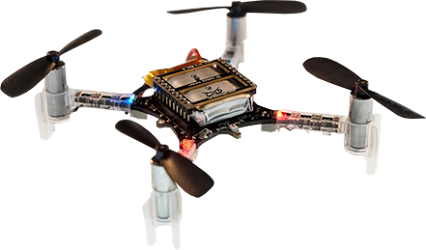
\includegraphics[width=.4\textwidth]{Images/crazyflie}
%\captionsetup[subfloat]{labelformat=empty}
%\subfloat[Picture from \cite{bitcraze}]{\hspace{\linewidth}}
%\caption{The CrazyFlie quadrotor from BitCraze}
%\label{fig:cf}
%\end{figure}

%%%%%%%%%%%%%%%%%%%%%%%%%%%%%%
%%%%%%%%%%% TWO FIGURES %%%%%%%%%%%
%%%%%%%%%%%%%%%%%%%%%%%%%%%%%%
%\begin{figure}[htbp]
%\centering
%\subfloat[Coarse Controller  ($K_p = 0.04,\  K_i = 0.008, \ K_d = 0.024$)]{\includegraphics[width=.45\textwidth]{Images/x_simple_PID}\label{fig:x_simple_PID_coarse}}
%\hspace{0.5cm}
%\subfloat[Fine Controller  ($K_p = 0.02,\  K_i = 0.004, \ K_d = 0.012$)]{\includegraphics[width=.45\textwidth]{Images/x_simple_PID_fine}\label{fig:x_simple_PID_fine}}
%\caption{X position for a simple PID controller}
%\label{fig:x_simple_PID}
%\end{figure}

%%%%%%%%%%%%%%%%%%%%%%%%%%%%%%
%%%%%%%%%%%%% TABLE %%%%%%%%%%%%%
%%%%%%%%%%%%%%%%%%%%%%%%%%%%%%
%\begin{table}[ht]
%\caption{X and Y controllers gains}
%\centering
%\begin{tabular}{|c|c|c|c|c|c|}
%\hline
%$\boldsymbol{K_{p,coarse}}$ & $\boldsymbol{K_{i,coarse}}$ & $\boldsymbol{K_{d,coarse}}$ &$\boldsymbol{K_{p,fine}}$ & $\boldsymbol{K_{i,fine}}$ & $\boldsymbol{K_{d,fine}}$ \\
%\hline
%0.04 & 0.008 & 0.024 & 0.02 & 0.004 & 0.024\\
%\hline
%\end{tabular}
%\label{tab:xy_param}
%\end{table}

%%%%%%%%%%%%%%%%%%%%%%%%%%%%%%
%%%%%%%%%%%%% CODE %%%%%%%%%%%%%
%%%%%%%%%%%%%%%%%%%%%%%%%%%%%%
%\lstset{
%commentstyle=\color{mygreen},
%stringstyle=\color{mymauve},
%keywordstyle=\color{blue},
%tabsize=2,
%frame=single,
%showstringspaces=false,
%basicstyle=\tiny
%}
%\lstinputlisting[language=Python]{Code/controlQuad.py}